\documentclass[a4paper,twoside,openright,11pt]{book}
% ==============================================================================
% L3S-Offshore-2 Frontend - Technical Documentation
% ==============================================================================

% --- Packages ---
\usepackage[T1]{fontenc}
\usepackage[utf8]{inputenc}
\usepackage[english]{babel}  % Changed to English for L3S

\usepackage{listings}
\usepackage{amssymb}
\usepackage{amsmath}
\usepackage{graphicx}
\usepackage{url}
\usepackage{hyperref}
\usepackage{xspace}
\usepackage{xcolor}
\usepackage{float}
\usepackage{booktabs}  % Better tables
\usepackage{caption}
\usepackage{subcaption}
\usepackage{tikz}
\usetikzlibrary{positioning, shapes.geometric, arrows.meta}

% --- Typography Fixes ---
\setlength{\emergencystretch}{3em}
\usepackage{etoolbox}
\apptocmd{\sloppy}{\hbadness 2000\relax}{}{}
\hyphenpenalty=5000
\tolerance=1000

% --- Graphics ---
\newcommand{\stdScaleFactor}{0.45}
\graphicspath{{contents/figures/}}

% --- Code Listings Configuration ---
\definecolor{codegreen}{rgb}{0,0.6,0}
\definecolor{codegray}{rgb}{0.5,0.5,0.5}
\definecolor{codepurple}{rgb}{0.58,0,0.82}
\definecolor{backcolour}{rgb}{0.95,0.95,0.92}

\lstdefinestyle{codestyle}{
    backgroundcolor=\color{backcolour},   
    commentstyle=\color{codegreen},
    keywordstyle=\color{blue},
    numberstyle=\tiny\color{codegray},
    stringstyle=\color{codepurple},
    basicstyle=\ttfamily\footnotesize,
    breakatwhitespace=false,         
    breaklines=true,                 
    captionpos=b,                    
    keepspaces=true,                 
    numbers=left,                    
    numbersep=5pt,                  
    showspaces=false,                
    showstringspaces=false,
    showtabs=false,                  
    tabsize=2,
    frame=single
}
\lstset{style=codestyle}

% TypeScript language definition
\lstdefinelanguage{TypeScript}{
  keywords={typeof, new, true, false, catch, function, return, null, catch, switch, var, let, const, if, in, while, do, else, case, break, class, export, boolean, throw, implements, import, this, interface, private, public, protected, async, await, readonly, type, enum, extends, static, void, never, any, unknown},
  keywordstyle=\color{blue}\bfseries,
  ndkeywords={Injectable, Component, Input, Output, ViewChild, HostListener, OnInit, OnDestroy, AfterViewInit, Observable, Subject, BehaviorSubject, Subscription},
  ndkeywordstyle=\color{codepurple}\bfseries,
  identifierstyle=\color{black},
  sensitive=true,
  comment=[l]{//},
  morecomment=[s]{/*}{*/},
  commentstyle=\color{codegreen}\ttfamily,
  stringstyle=\color{red}\ttfamily,
  morestring=[b]',
  morestring=[b]"
}

% JSON language definition
\lstdefinelanguage{json}{
  basicstyle=\ttfamily\footnotesize,
  stringstyle=\color{red},
  numbers=left,
  numberstyle=\tiny\color{codegray},
  stepnumber=1,
  numbersep=5pt,
  showstringspaces=false,
  breaklines=true,
  morestring=[b]"
}

% YAML language definition
\lstdefinelanguage{yaml}{
  keywords={true,false,null,y,n},
  keywordstyle=\color{blue}\bfseries,
  basicstyle=\ttfamily\footnotesize,
  sensitive=false,
  comment=[l]{\#},
  commentstyle=\color{codegreen}\ttfamily,
  stringstyle=\color{red}\ttfamily,
  morestring=[b]',
  morestring=[b]"
}

% Docker language definition (simplified shell)
\lstdefinelanguage{docker}{
  keywords={FROM, RUN, CMD, LABEL, EXPOSE, ENV, ADD, COPY, ENTRYPOINT, VOLUME, USER, WORKDIR, ARG, ONBUILD, STOPSIGNAL, HEALTHCHECK, SHELL, AS},
  keywordstyle=\color{blue}\bfseries,
  basicstyle=\ttfamily\footnotesize,
  sensitive=false,
  comment=[l]{\#},
  commentstyle=\color{codegreen}\ttfamily,
  stringstyle=\color{red}\ttfamily,
  morestring=[b]',
  morestring=[b]"
}

% --- L3S Project Style ---
\usepackage{l3s-project-doc}

% --- Project Metadata ---
\projectname{L3S-Offshore-2 Frontend}
\projectsubtitle{Web-based Petri Net Visualization and Simulation Tool}
\institution{L3S Research Center}
\researchgroup{Knowledge-Based Systems Group}
\university{Leibniz Universität Hannover}
\authorname{Martin Krauser}
\authoremail{martin.krauser@stud.uni-hannover.de}
\supervisor{Shengrui Peng}
\supervisoremail{}
\projectperiod{March 2025 -- January 2026}
\docversion{1.0}
\docdate{November 2025}
\city{Hannover}

% --- Hyperref Configuration ---
\hypersetup{
    colorlinks=true,
    linkcolor=blue,
    filecolor=magenta,      
    urlcolor=cyan,
    pdftitle={L3S-Offshore-2 Frontend Documentation},
    pdfauthor={Martin Krauser},
}

% ==============================================================================
\begin{document}

\frontmatter

\maketitle

\clearpage
\makedocinfo

\clearpage
\chapter*{Abstract}
\addcontentsline{toc}{chapter}{Abstract}

This document provides comprehensive technical documentation for the L3S-Offshore-2 Frontend, a web-based application for Petri net visualization, manipulation, and simulation. The frontend was developed as part of the L3S-Offshore-2 research project at the L3S Research Center, Leibniz Universität Hannover.

The application is built using Angular and provides the following core capabilities:
\begin{itemize}
    \item \textbf{Visualization:} Interactive rendering of Petri nets from PNML files with automatic layout algorithms (Sugiyama)
    \item \textbf{Manipulation:} Drag-and-drop editing of places, transitions, and arcs with real-time token modification
    \item \textbf{Simulation:} Step-by-step and automated playback of firing sequences with transition highlighting
    \item \textbf{Analysis:} Display of place invariants and transition firing statistics from multi-run simulations
    \item \textbf{Offshore Scheduling:} Dedicated parameter interface for offshore wind farm installation scheduling models
\end{itemize}

The documentation covers the system architecture, key implementation details, deployment procedures, and provides guidance for future development and maintenance.

\clearpage


\tableofcontents
\listoffigures
\listoftables

\mainmatter

% Part I: Introduction and Background
\input{contents/01-introduction.tex}
\input{contents/02-fundamentals.tex}

% Part II: Core Concepts (based on Markdown Manual structure)
\chapter{UI Service: User Interface State Management}
\label{chap:ui-service}

This chapter introduces the \texttt{UiService}, the central component responsible for managing the application's user interface state. Understanding this service is fundamental, as it dictates what the user sees and how the application responds to their interactions.

\section{Problem Statement}
\label{sec:ui-problem}

Consider a common user action: \textbf{switching tabs}. The application has different tabs such as ``Build'', ``Simulation'', and ``Analyze''. When the user clicks on the ``Simulation'' tab:

\begin{enumerate}
    \item The clicked button must inform the rest of the application: ``We are now in Simulation mode.''
    \item The main drawing area must update to show simulation-specific elements (e.g., animated token flow) instead of editing tools.
    \item Other UI components (sidebars, status messages) must reflect the new ``Simulation'' context.
\end{enumerate}

Without a centralized state management approach, every component would need to independently track the current tab, leading to:
\begin{itemize}
    \item \textbf{Inconsistency}: Components might display conflicting states
    \item \textbf{Tight coupling}: Components must directly communicate with each other
    \item \textbf{Maintenance burden}: Changes require updates across multiple files
\end{itemize}

The \texttt{UiService} solves this by being the \textbf{single source of truth} for what the user interface is currently displaying or doing.

\section{Conceptual Overview}
\label{sec:ui-concept}

Think of the \texttt{UiService} as the application's \textbf{control panel} or \textbf{dashboard}. It maintains critical information about the UI state:

\begin{itemize}
    \item \textbf{Active tab}: Which workflow is currently visible (Build, Simulation, Analyze, etc.)
    \item \textbf{Selected tool}: Which editing tool is active (Add Place, Move, Delete, etc.)
    \item \textbf{Simulation speed}: The playback rate for animation
    \item \textbf{Editor format}: Whether the Code tab shows JSON or PNML
\end{itemize}

Other components \textit{subscribe} to the \texttt{UiService}---similar to subscribing to a notification channel. When the service announces a change (e.g., ``The active tab is now Simulation!''), all subscribed components automatically react, ensuring the application remains responsive and consistent.

\section{State Definitions}
\label{sec:ui-states}

The application defines its UI states using TypeScript enums, providing clear, human-readable names instead of magic numbers.

\begin{lstlisting}[language=TypeScript, caption={UI state enums (src/app/tr-enums/ui-state.ts)}]
/**
 * Represents the currently active tab in the application.
 * Each tab corresponds to a different workflow/mode.
 */
export enum TabState {
    Build,       // Graphical editing of Petri net elements
    Simulation,  // Playback and animation of firing sequences
    Save,        // Export options (PNG, SVG, JSON, PNML)
    Code,        // Text-based editing of PNML/JSON
    Analyze,     // Place invariants and analysis results
    Offshore,    // Domain-specific parameter configuration
}

/**
 * Represents the currently selected editing tool in Build mode.
 */
export enum ButtonState {
    Blitz,       // Quick-add mode
    Place,       // Add a new place (circle)
    Transition,  // Add a new transition (rectangle)
    Move,        // Drag elements to reposition
    Arc,         // Connect places and transitions
    Delete,      // Remove elements
    // ... additional tools ...
}

/**
 * Format for the Code tab editor.
 */
export enum CodeEditorFormat {
    JSON,        // Custom JSON format
    PNML,        // Standard PNML XML format
}
\end{lstlisting}

Using enums like \texttt{TabState.Simulation} is far more readable and maintainable than remembering that ``tab state 1'' means simulation mode.

\section{The UiService Implementation}
\label{sec:ui-implementation}

The \texttt{UiService} class holds the actual state variables and provides reactive streams (Observables) that notify listeners of changes.

\begin{lstlisting}[language=TypeScript, caption={UiService core implementation (src/app/tr-services/ui.service.ts)}]
import { Injectable } from '@angular/core';
import { BehaviorSubject, Observable } from 'rxjs';
import { ButtonState, CodeEditorFormat, TabState } from '../tr-enums/ui-state';

@Injectable({
    providedIn: 'root', // Singleton: one instance for the entire application
})
export class UiService {
    // =========================================================================
    // TAB STATE MANAGEMENT
    // =========================================================================
    
    /** Private variable holding the current tab */
    private _tab: TabState = TabState.Build;
    
    /** 
     * BehaviorSubject: a special Observable that remembers its last value.
     * New subscribers immediately receive the current state.
     */
    private _tab$ = new BehaviorSubject<TabState>(this._tab);
    
    /** Public Observable for components to subscribe to */
    public tab$: Observable<TabState> = this._tab$.asObservable();

    /** Getter: read the current tab synchronously */
    public get tab(): TabState {
        return this._tab;
    }

    /** 
     * Setter: update the current tab.
     * Automatically notifies all subscribers via the BehaviorSubject.
     */
    public set tab(value: TabState) {
        if (this._tab !== value) {
            console.log(`[UiService] Tab changed: ${TabState[this._tab]} -> ${TabState[value]}`);
            this._tab = value;
            this._tab$.next(value); // Broadcast to all subscribers
        }
    }

    // =========================================================================
    // SIMULATION SPEED MANAGEMENT
    // =========================================================================
    
    private _simulationSpeed$ = new BehaviorSubject<number>(1); // Default: 1x speed
    public simulationSpeed$: Observable<number> = this._simulationSpeed$.asObservable();

    /** Update the simulation playback speed multiplier */
    public setSimulationSpeed(speed: number): void {
        this._simulationSpeed$.next(speed);
    }

    /** Get the current speed multiplier synchronously */
    public getAnimationSpeedMultiplier(): number {
        return this._simulationSpeed$.getValue();
    }

    // ... additional state management for tools, editor format, etc. ...
}
\end{lstlisting}

\subsection{Key Concepts Explained}

\begin{description}
    \item[@Injectable(\{providedIn: 'root'\})] Makes \texttt{UiService} a \textbf{singleton}---only one instance exists throughout the application. This ensures all components share the same state.
    
    \item[BehaviorSubject<T>] A special RxJS type that:
    \begin{itemize}
        \item Always holds a current value
        \item Immediately emits the current value to new subscribers
        \item Broadcasts new values to all active subscribers when \texttt{.next()} is called
    \end{itemize}
    
    \item[Getter/Setter pattern] The \texttt{get tab()} and \texttt{set tab()} methods provide a clean API. The setter automatically calls \texttt{\_tab\$.next(value)} to notify subscribers.
\end{description}

\section{Usage Patterns}
\label{sec:ui-usage}

\subsection{Changing the UI State}

When a user clicks a tab button, the \texttt{ButtonBarComponent} updates the \texttt{UiService}:

\begin{lstlisting}[language=TypeScript, caption={Setting the tab state (ButtonBarComponent)}]
import { Component } from '@angular/core';
import { UiService } from 'src/app/tr-services/ui.service';
import { TabState } from 'src/app/tr-enums/ui-state';

@Component({ /* ... */ })
export class ButtonBarComponent {
    constructor(protected uiService: UiService) {}

    /**
     * Called when user clicks a tab button.
     * Updates the UiService, which broadcasts to all subscribers.
     */
    tabClicked(tabName: string): void {
        switch (tabName.toLowerCase()) {
            case 'build':
                this.uiService.tab = TabState.Build;
                break;
            case 'simulation':
                this.uiService.tab = TabState.Simulation;
                break;
            case 'analyze':
                this.uiService.tab = TabState.Analyze;
                break;
            // ... other tabs ...
        }
    }
}
\end{lstlisting}

\subsection{Listening to UI State Changes}

Components that need to react to state changes \textit{subscribe} to the observable:

\begin{lstlisting}[language=TypeScript, caption={Subscribing to tab changes (AppComponent)}]
import { Component, OnInit, OnDestroy } from '@angular/core';
import { Subscription } from 'rxjs';
import { UiService } from './tr-services/ui.service';
import { TabState } from './tr-enums/ui-state';

@Component({ /* ... */ })
export class AppComponent implements OnInit, OnDestroy {
    private tabSubscription: Subscription;

    constructor(protected uiService: UiService) {}

    ngOnInit(): void {
        // Subscribe to tab changes
        this.tabSubscription = this.uiService.tab$.subscribe(currentTab => {
            console.log('Current tab:', TabState[currentTab]);
            
            // React to the change
            if (currentTab === TabState.Simulation) {
                this.showSimulationControls();
            } else {
                this.hideSimulationControls();
            }
        });
    }

    ngOnDestroy(): void {
        // Always unsubscribe to prevent memory leaks
        this.tabSubscription?.unsubscribe();
    }
    
    // ...
}
\end{lstlisting}

The \texttt{\$} suffix on \texttt{tab\$} is a common Angular/RxJS convention indicating that the property is an Observable (a ``stream'' of values over time).

\section{Data Flow Visualization}
\label{sec:ui-flow}

The following sequence illustrates what happens when a user switches tabs:

\begin{figure}[htb]
    \centering
    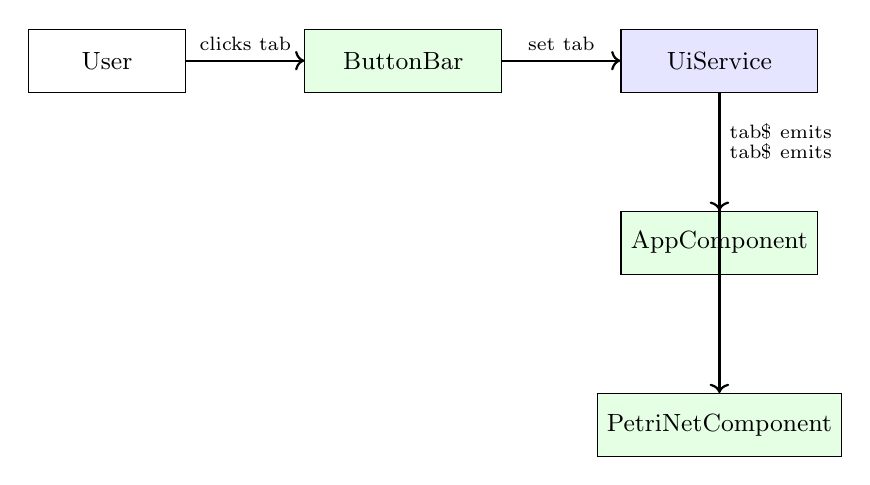
\begin{tikzpicture}[
        node distance=1.5cm,
        every node/.style={font=\small},
        actor/.style={rectangle, draw, minimum width=2cm, minimum height=0.8cm},
        service/.style={rectangle, draw, fill=blue!10, minimum width=2.5cm, minimum height=0.8cm},
        component/.style={rectangle, draw, fill=green!10, minimum width=2.5cm, minimum height=0.8cm},
    ]
        % Nodes
        \node[actor] (user) {User};
        \node[component, right=of user] (buttonbar) {ButtonBar};
        \node[service, right=of buttonbar] (uiservice) {UiService};
        \node[component, below=of uiservice] (app) {AppComponent};
        \node[component, below=of app] (petrinet) {PetriNetComponent};
        
        % Arrows
        \draw[->, thick] (user) -- node[above] {\scriptsize clicks tab} (buttonbar);
        \draw[->, thick] (buttonbar) -- node[above] {\scriptsize set tab} (uiservice);
        \draw[->, thick] (uiservice) -- node[right] {\scriptsize tab\$ emits} (app);
        \draw[->, thick] (uiservice.south) -- ++(0,-0.5) -| node[near start, right] {\scriptsize tab\$ emits} (petrinet.north);
        
    \end{tikzpicture}
    \caption{Tab switching data flow through UiService}
    \label{fig:ui-service-flow}
\end{figure}

\begin{enumerate}
    \item \textbf{User Action}: User clicks the ``Simulation'' tab button
    \item \textbf{State Update}: \texttt{ButtonBarComponent} sets \texttt{uiService.tab = TabState.Simulation}
    \item \textbf{Internal Update}: \texttt{UiService} updates \texttt{\_tab} and calls \texttt{\_tab\$.next(value)}
    \item \textbf{Broadcast}: All subscribers to \texttt{tab\$} receive the new value
    \item \textbf{Component Reactions}: 
    \begin{itemize}
        \item \texttt{AppComponent} shows the simulation timeline
        \item \texttt{PetriNetComponent} enables transition highlighting and hides build tools
    \end{itemize}
\end{enumerate}

\section{Practical Example: Tab-Aware Behavior}
\label{sec:ui-example}

The \texttt{PetriNetComponent} demonstrates how components use \texttt{tab\$} to conditionally enable features:

\begin{lstlisting}[language=TypeScript, caption={Tab-aware component behavior}]
import { Component, OnInit } from '@angular/core';
import { UiService } from 'src/app/tr-services/ui.service';
import { TabState } from 'src/app/tr-enums/ui-state';

@Component({ /* ... */ })
export class PetriNetComponent implements OnInit {
    private previousTab: TabState;

    constructor(private uiService: UiService) {}

    ngOnInit(): void {
        this.uiService.tab$.subscribe(currentTab => {
            // Leaving Simulation tab: clean up highlights and reset tokens
            if (this.previousTab === TabState.Simulation && currentTab !== TabState.Simulation) {
                this.clearAllHighlights();
                this.resetTokensToBaseline();
            }
            
            // Entering Simulation tab: save baseline marking
            if (currentTab === TabState.Simulation && this.previousTab !== TabState.Simulation) {
                this.saveBaselineMarking();
            }
            
            // Entering Build tab: enable editing tools
            if (currentTab === TabState.Build) {
                this.enableDragAndDrop();
                this.showEditingHandles();
            } else {
                this.disableDragAndDrop();
                this.hideEditingHandles();
            }
            
            this.previousTab = currentTab;
        });
    }
    
    // ... helper methods ...
}
\end{lstlisting}

This pattern ensures that:
\begin{itemize}
    \item Simulation highlights are cleared when leaving the Simulation tab
    \item Token counts are reset to their initial values
    \item Editing tools are only active in Build mode
\end{itemize}

\section{Summary}
\label{sec:ui-summary}

The \texttt{UiService} is the application's \textbf{control panel}, centralizing all UI state management:

\begin{itemize}
    \item Uses \textbf{TypeScript enums} for type-safe state definitions
    \item Employs \textbf{BehaviorSubject} for reactive state broadcasting
    \item Provides \textbf{getter/setter} methods for clean state access
    \item Enables \textbf{decoupled components} that react to state changes without direct communication
\end{itemize}

Understanding the \texttt{UiService} is essential because it controls what the user experiences. In the next chapter, we will examine the \textbf{Petri Net Elements}---the actual data objects (places, transitions, arcs) that the UI displays and manipulates.

\chapter{Petri Net Elements: Core Data Model}
\label{chap:petri-net-elements}

In the previous chapter, we explored the \texttt{UiService}, which manages \textit{what} the user is doing. This chapter focuses on \textit{what} the user is working with: the \textbf{Petri Net Elements}---the fundamental data objects that define the structure and behavior of any Petri net in our application.

\section{Problem Statement}
\label{sec:elements-problem}

To model a process like ``sending a letter,'' we need to represent:
\begin{itemize}
    \item \textbf{States}: The letter is unstamped, stamped, or mailed
    \item \textbf{Actions}: Stamp the letter, mail the letter
    \item \textbf{Flow}: How actions connect states
\end{itemize}

The \textbf{Petri Net Elements} are the fundamental building blocks that answer these questions. They are the ``nouns'' (states/conditions), ``verbs'' (actions/events), and ``arrows'' (connections) of our process models.

\section{Core Building Blocks}
\label{sec:elements-overview}

Petri nets consist of three element types:

\begin{table}[htb]
    \centering
    \begin{tabular}{llll}
        \toprule
        \textbf{Element} & \textbf{Visual} & \textbf{Represents} & \textbf{Analogy} \\
        \midrule
        Place & Circle ($\bigcirc$) & States, conditions, resources & Container, location \\
        Transition & Rectangle ($\square$) & Events, actions, activities & Action, step, verb \\
        Arc & Arrow ($\rightarrow$) & Causal links, token flow & Pathway, connection \\
        \bottomrule
    \end{tabular}
    \caption{The three core Petri net element types}
    \label{tab:petri-elements}
\end{table}

\section{Places: State Containers}
\label{sec:places}

Places are represented as circles. They hold \textbf{tokens} (visualized as small dots inside the circle) and represent conditions, resources, or states.

\begin{itemize}
    \item A place with tokens indicates that the condition is \textbf{active} or the resource is \textbf{available}
    \item Example: A place named ``Coffee Beans'' with 5 tokens means 5 portions are ready
\end{itemize}

\begin{lstlisting}[language=TypeScript, caption={Place class definition (src/app/tr-classes/petri-net/place.ts)}]
import { Point } from './point';
import { Node } from 'src/app/tr-interfaces/petri-net/node';

/**
 * Represents a Place in a Petri net.
 * Places hold tokens and model conditions/states.
 */
export class Place implements Node {
    /** Number of tokens currently in this place */
    token: number;
    
    /** Position on the canvas (x, y coordinates) */
    position: Point;
    
    /** Unique identifier, e.g., 'p1', 'p2' */
    id: string;
    
    /** Optional display name, e.g., 'Coffee Beans' */
    label?: string;

    constructor(token: number, position: Point, id: string, label?: string) {
        this.token = token;
        this.position = position;
        this.id = id;
        this.label = label;
    }

    /**
     * Check if this place has at least the required number of tokens.
     * Used for determining if connected transitions can fire.
     */
    hasEnoughTokens(required: number): boolean {
        return this.token >= required;
    }

    /**
     * Consume tokens from this place (called when a transition fires).
     */
    removeTokens(count: number): void {
        this.token = Math.max(0, this.token - count);
    }

    /**
     * Add tokens to this place (called when a transition fires).
     */
    addTokens(count: number): void {
        this.token += count;
    }
}
\end{lstlisting}

\section{Transitions: Action Nodes}
\label{sec:transitions}

Transitions are represented as rectangles. They model events or actions that can occur when their input conditions are met. Transitions do not hold tokens; instead, they \textbf{fire} (execute) when enabled.

\begin{lstlisting}[language=TypeScript, caption={Transition class definition (src/app/tr-classes/petri-net/transition.ts)}]
import { Point } from './point';
import { Node } from 'src/app/tr-interfaces/petri-net/node';
import { Arc } from './arc';

/**
 * Represents a Transition in a Petri net.
 * Transitions model events/actions and connect input places to output places.
 */
export class Transition implements Node {
    /** Position on the canvas */
    position: Point;
    
    /** Unique identifier, e.g., 't1', 't2' */
    id: string;
    
    /** Optional display name, e.g., 'Grind Beans' */
    label?: string;
    
    /** Arcs coming INTO this transition (from input places) */
    preArcs: Arc[] = [];
    
    /** Arcs going OUT OF this transition (to output places) */
    postArcs: Arc[] = [];

    constructor(position: Point, id: string, label?: string) {
        this.position = position;
        this.id = id;
        this.label = label;
    }

    /**
     * Check if this transition is enabled (can fire).
     * A transition is enabled when ALL input places have enough tokens.
     */
    isEnabled(): boolean {
        return this.preArcs.every(arc => {
            const place = arc.from as Place;
            return place.hasEnoughTokens(Math.abs(arc.weight));
        });
    }

    /**
     * Fire this transition: consume tokens from inputs, produce tokens in outputs.
     */
    fire(): void {
        if (!this.isEnabled()) {
            console.warn(`Transition ${this.id} cannot fire: not enabled`);
            return;
        }

        // Consume tokens from input places
        this.preArcs.forEach(arc => {
            const place = arc.from as Place;
            place.removeTokens(Math.abs(arc.weight));
        });

        // Produce tokens in output places
        this.postArcs.forEach(arc => {
            const place = arc.to as Place;
            place.addTokens(Math.abs(arc.weight));
        });
    }

    /** Add an incoming arc (from a place to this transition) */
    appendPreArc(arc: Arc): void {
        this.preArcs.push(arc);
    }

    /** Add an outgoing arc (from this transition to a place) */
    appendPostArc(arc: Arc): void {
        this.postArcs.push(arc);
    }
}
\end{lstlisting}

\subsection{Firing Rules}

A transition $t$ is \textbf{enabled} when all input places have sufficient tokens:
\[
\forall p \in \bullet t: M(p) \geq W(p, t)
\]

When an enabled transition fires:
\begin{enumerate}
    \item Tokens are \textbf{consumed} from each input place according to the arc weight
    \item Tokens are \textbf{produced} in each output place according to the arc weight
\end{enumerate}

\section{Arcs: Flow Connections}
\label{sec:arcs}

Arcs are directed edges connecting places to transitions or transitions to places. They define the \textbf{flow} of tokens through the net.

\begin{itemize}
    \item \textbf{Place $\rightarrow$ Transition}: Tokens from the place are required for the transition to fire
    \item \textbf{Transition $\rightarrow$ Place}: When the transition fires, tokens are produced in the place
\end{itemize}

\begin{lstlisting}[language=TypeScript, caption={Arc class definition (src/app/tr-classes/petri-net/arc.ts)}]
import { Node } from 'src/app/tr-interfaces/petri-net/node';
import { Point } from './point';

/**
 * Represents an Arc (directed edge) connecting nodes in a Petri net.
 * Arcs always connect a Place to a Transition or a Transition to a Place.
 */
export class Arc {
    /** Starting node (either Place or Transition) */
    from: Node;
    
    /** Ending node (either Place or Transition) */
    to: Node;
    
    /** 
     * Arc weight: how many tokens are moved.
     * Default is 1. A weight of 2 means 2 tokens are consumed/produced.
     */
    weight: number;
    
    /** 
     * Optional anchor points for curved arcs.
     * Allows visual bending of the arc on the canvas.
     */
    anchors: Point[];

    constructor(from: Node, to: Node, weight: number = 1, anchors: Point[] = []) {
        this.from = from;
        this.to = to;
        this.weight = weight;
        this.anchors = anchors;
    }

    /**
     * Get the source position for drawing.
     */
    getSourcePosition(): Point {
        return this.from.position;
    }

    /**
     * Get the target position for drawing.
     */
    getTargetPosition(): Point {
        return this.to.position;
    }
}
\end{lstlisting}

\section{The Node Interface}
\label{sec:node-interface}

Both \texttt{Place} and \texttt{Transition} implement the \texttt{Node} interface, which defines their common properties:

\begin{lstlisting}[language=TypeScript, caption={Node interface (src/app/tr-interfaces/petri-net/node.ts)}]
import { Point } from 'src/app/tr-classes/petri-net/point';

/**
 * Common interface for all Petri net nodes (Places and Transitions).
 * Enables arcs to connect any type of node generically.
 */
export interface Node {
    /** Position on the canvas */
    position: Point;
    
    /** Unique identifier within the net */
    id: string;
    
    /** Optional human-readable label */
    label?: string;
}
\end{lstlisting}

This interface allows the \texttt{Arc} class to work with both places and transitions without knowing the specific type.

\section{The Point Class}
\label{sec:point-class}

All elements use the \texttt{Point} class to define their canvas coordinates:

\begin{lstlisting}[language=TypeScript, caption={Point class (src/app/tr-classes/petri-net/point.ts)}]
/**
 * Represents a 2D coordinate on the canvas.
 */
export class Point {
    constructor(
        public x: number,
        public y: number,
    ) {}

    /**
     * Calculate distance to another point.
     */
    distanceTo(other: Point): number {
        const dx = this.x - other.x;
        const dy = this.y - other.y;
        return Math.sqrt(dx * dx + dy * dy);
    }

    /**
     * Create a copy of this point.
     */
    clone(): Point {
        return new Point(this.x, this.y);
    }
}
\end{lstlisting}

\section{Practical Example: Building a Simple Net}
\label{sec:elements-example}

Let's create a simple ``sending a letter'' Petri net programmatically:

\begin{lstlisting}[language=TypeScript, caption={Creating a Petri net in code}]
import { Place } from 'src/app/tr-classes/petri-net/place';
import { Transition } from 'src/app/tr-classes/petri-net/transition';
import { Arc } from 'src/app/tr-classes/petri-net/arc';
import { Point } from 'src/app/tr-classes/petri-net/point';

// 1. Create places (states)
const unstampedLetter = new Place(
    1,                      // Initial tokens: 1 letter ready
    new Point(100, 100),    // Position on canvas
    'p1',                   // Unique ID
    'Unstamped Letter'      // Label
);

const stampedLetter = new Place(
    0,                      // No tokens initially
    new Point(300, 100),
    'p2',
    'Stamped Letter'
);

const mailedLetter = new Place(
    0,
    new Point(500, 100),
    'p3',
    'Mailed Letter'
);

// 2. Create transitions (actions)
const stampAction = new Transition(
    new Point(200, 100),
    't1',
    'Stamp Letter'
);

const mailAction = new Transition(
    new Point(400, 100),
    't2',
    'Mail Letter'
);

// 3. Connect with arcs
const arc1 = new Arc(unstampedLetter, stampAction);  // p1 -> t1
const arc2 = new Arc(stampAction, stampedLetter);    // t1 -> p2
const arc3 = new Arc(stampedLetter, mailAction);     // p2 -> t2
const arc4 = new Arc(mailAction, mailedLetter);      // t2 -> p3

// 4. Register arcs with transitions
stampAction.appendPreArc(arc1);
stampAction.appendPostArc(arc2);
mailAction.appendPreArc(arc3);
mailAction.appendPostArc(arc4);

// 5. Check which transitions are enabled
console.log('Stamp enabled:', stampAction.isEnabled());  // true (p1 has token)
console.log('Mail enabled:', mailAction.isEnabled());    // false (p2 has no token)

// 6. Fire the stamp transition
stampAction.fire();
console.log('After stamping:');
console.log('  p1 tokens:', unstampedLetter.token);  // 0
console.log('  p2 tokens:', stampedLetter.token);    // 1
console.log('  Mail enabled:', mailAction.isEnabled()); // true
\end{lstlisting}

\textbf{Output:}
\begin{verbatim}
Stamp enabled: true
Mail enabled: false
After stamping:
  p1 tokens: 0
  p2 tokens: 1
  Mail enabled: true
\end{verbatim}

\section{Class Diagram}
\label{sec:elements-diagram}

\begin{figure}[htb]
    \centering
    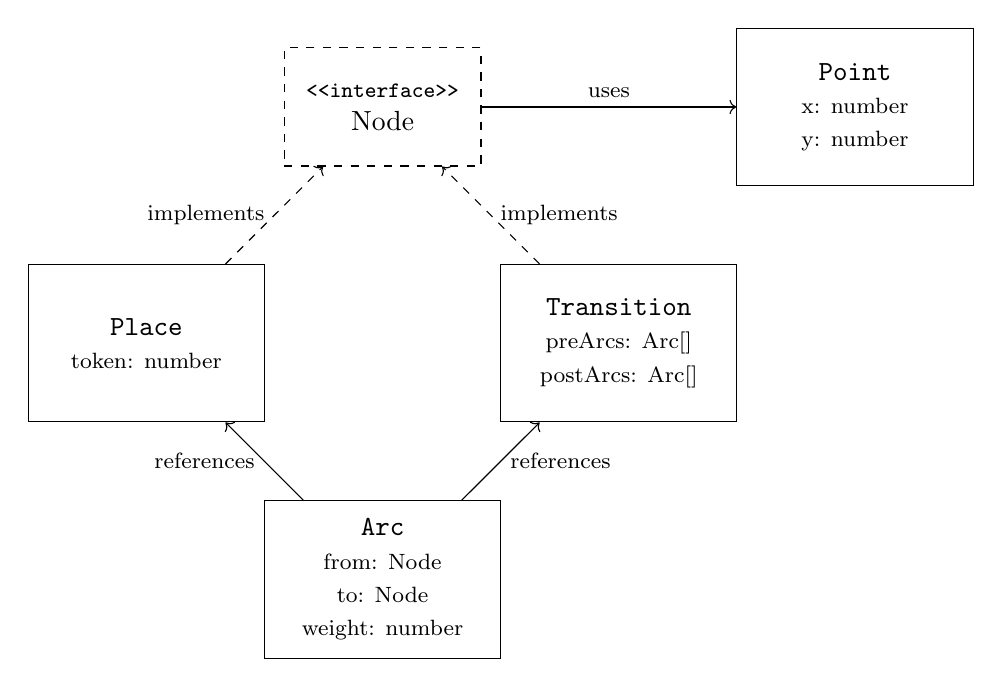
\begin{tikzpicture}[
        class/.style={rectangle, draw, minimum width=3cm, minimum height=2cm, align=center},
        interface/.style={rectangle, draw, dashed, minimum width=2.5cm, minimum height=1.5cm, align=center},
    ]
        % Classes
        \node[interface] (node) at (0, 3) {\footnotesize \texttt{<<interface>>}\\Node};
        \node[class] (place) at (-3, 0) {\texttt{Place}\\{\footnotesize token: number}};
        \node[class] (transition) at (3, 0) {\texttt{Transition}\\{\footnotesize preArcs: Arc[]}\\{\footnotesize postArcs: Arc[]}};
        \node[class] (arc) at (0, -3) {\texttt{Arc}\\{\footnotesize from: Node}\\{\footnotesize to: Node}\\{\footnotesize weight: number}};
        \node[class] (point) at (6, 3) {\texttt{Point}\\{\footnotesize x: number}\\{\footnotesize y: number}};
        
        % Relationships
        \draw[->, dashed] (place) -- (node) node[midway, left] {\footnotesize implements};
        \draw[->, dashed] (transition) -- (node) node[midway, right] {\footnotesize implements};
        \draw[->] (arc) -- (place) node[midway, left] {\footnotesize references};
        \draw[->] (arc) -- (transition) node[midway, right] {\footnotesize references};
        \draw[->] (node) -- (point) node[midway, above] {\footnotesize uses};
    \end{tikzpicture}
    \caption{Petri net element class relationships}
    \label{fig:elements-class-diagram}
\end{figure}

\section{Summary}
\label{sec:elements-summary}

The \textbf{Petri Net Elements} are the fundamental data objects that define any Petri net:

\begin{itemize}
    \item \textbf{Place}: Holds tokens, represents states/conditions
    \item \textbf{Transition}: Represents actions, fires when enabled
    \item \textbf{Arc}: Connects places and transitions, defines token flow
    \item \textbf{Point}: Stores canvas coordinates for positioning
    \item \textbf{Node interface}: Common contract for places and transitions
\end{itemize}

These objects are the ``things'' you manipulate when designing a Petri net. But how does the application manage a \textit{collection} of these elements? How does it track all places, transitions, and arcs in your entire net? That's the role of the \textbf{Data Service}, which we explore in the next chapter.

\chapter{Data Service: Central Data Store}
\label{chap:data-service}

The previous chapter introduced the \textbf{Petri Net Elements}---the individual building blocks (places, transitions, arcs) of our models. This chapter focuses on the \textbf{Data Service}, which acts as the central repository for all these elements and ensures the entire application stays synchronized.

\section{Problem Statement}
\label{sec:data-problem}

Consider what happens when you \textbf{add a new Place} to your Petri net:

\begin{enumerate}
    \item You drag a ``Place'' icon onto the canvas
    \item The application creates a new \texttt{Place} object in memory
    \item This new place must be \textbf{stored} somewhere accessible
    \item The \textbf{drawing component} must know about it to render it
    \item The \textbf{save function} must include it when exporting
    \item The \textbf{simulation engine} must consider it when calculating enabled transitions
\end{enumerate}

Without a central data store, every component would maintain its own list of elements. If one component adds a place, how do the others know? If one deletes an arc, how do the others update? This would lead to:

\begin{itemize}
    \item \textbf{Inconsistent state}: Different components showing different data
    \item \textbf{Complex synchronization}: Manual coordination between components
    \item \textbf{Bug-prone code}: Easy to forget updating one of many lists
\end{itemize}

The \texttt{DataService} solves this by being the \textbf{single source of truth} for all Petri net data.

\section{Conceptual Overview}
\label{sec:data-concept}

Think of the \texttt{DataService} as the application's \textbf{central brain} or \textbf{shared whiteboard}. It maintains:

\begin{itemize}
    \item \textbf{All Places}: Their tokens, positions, IDs, and labels
    \item \textbf{All Transitions}: Their positions, IDs, labels, and connected arcs
    \item \textbf{All Arcs}: Source/target nodes, weights, and anchor points
    \item \textbf{All Actions}: Unique labels used by transitions
\end{itemize}

When anything changes, the \texttt{DataService}:
\begin{enumerate}
    \item Updates its internal records
    \item \textbf{Broadcasts} the change to all interested components
\end{enumerate}

This ensures every part of the application sees the same, up-to-date data.

\section{Implementation}
\label{sec:data-implementation}

\begin{lstlisting}[language=TypeScript, caption={DataService core implementation (src/app/tr-services/data.service.ts)}]
import { Injectable } from '@angular/core';
import { Subject, Observable } from 'rxjs';
import { Arc } from '../tr-classes/petri-net/arc';
import { Place } from '../tr-classes/petri-net/place';
import { Transition } from '../tr-classes/petri-net/transition';

/**
 * Payload emitted when data changes.
 * fitContent: if true, the UI should re-center the view on the net.
 */
interface DataChangedPayload {
    fitContent: boolean;
}

@Injectable({
    providedIn: 'root', // Singleton: one instance for entire application
})
export class DataService {
    // =========================================================================
    // PRIVATE DATA STORAGE
    // =========================================================================
    
    /** All places in the current Petri net */
    private _places: Place[] = [];
    
    /** All transitions in the current Petri net */
    private _transitions: Transition[] = [];
    
    /** All arcs connecting places and transitions */
    private _arcs: Arc[] = [];
    
    /** Unique action labels used by transitions */
    private _actions: string[] = [];

    // =========================================================================
    // CHANGE NOTIFICATION
    // =========================================================================
    
    /**
     * Subject for broadcasting data changes.
     * Components subscribe to be notified when the Petri net is modified.
     */
    private dataChangedSubject = new Subject<DataChangedPayload>();
    
    /** Public observable for subscribing to data changes */
    public dataChanged$: Observable<DataChangedPayload> = 
        this.dataChangedSubject.asObservable();

    // =========================================================================
    // GETTERS: Read current data
    // =========================================================================
    
    getPlaces(): Place[] { return this._places; }
    getTransitions(): Transition[] { return this._transitions; }
    getArcs(): Arc[] { return this._arcs; }
    getActions(): string[] { return this._actions; }

    // =========================================================================
    // SETTERS: Replace entire collections (used when loading files)
    // =========================================================================
    
    set places(value: Place[]) { this._places = value; }
    set transitions(value: Transition[]) { this._transitions = value; }
    set arcs(value: Arc[]) { this._arcs = value; }
    set actions(value: string[]) { this._actions = value; }

    // =========================================================================
    // MODIFICATION METHODS
    // =========================================================================

    /**
     * Add a new place to the Petri net.
     */
    addPlace(place: Place): void {
        this._places.push(place);
        this.triggerDataChanged();
    }

    /**
     * Remove a place and all its connected arcs.
     */
    removePlace(deletablePlace: Place): void {
        // First, remove all arcs connected to this place
        const connectedArcs = this._arcs.filter(
            arc => arc.from === deletablePlace || arc.to === deletablePlace
        );
        connectedArcs.forEach(arc => this.removeArc(arc));

        // Then remove the place itself
        this._places = this._places.filter(place => place !== deletablePlace);
        
        this.triggerDataChanged();
    }

    /**
     * Add a new transition to the Petri net.
     */
    addTransition(transition: Transition): void {
        this._transitions.push(transition);
        this.triggerDataChanged();
    }

    /**
     * Remove a transition and all its connected arcs.
     */
    removeTransition(deletableTransition: Transition): void {
        // Remove connected arcs
        const connectedArcs = this._arcs.filter(
            arc => arc.from === deletableTransition || arc.to === deletableTransition
        );
        connectedArcs.forEach(arc => this.removeArc(arc));

        // Remove the transition
        this._transitions = this._transitions.filter(t => t !== deletableTransition);
        
        this.triggerDataChanged();
    }

    /**
     * Connect two nodes with a new arc.
     * Validates that the connection follows Petri net rules:
     * - Place -> Transition (input arc)
     * - Transition -> Place (output arc)
     */
    connectNodes(from: Node, to: Node): Arc | null {
        // Validate: cannot connect Place to Place or Transition to Transition
        if (from instanceof Place && to instanceof Place) {
            console.error('Cannot connect Place to Place');
            return null;
        }
        if (from instanceof Transition && to instanceof Transition) {
            console.error('Cannot connect Transition to Transition');
            return null;
        }

        const arc = new Arc(from, to, 1);
        this._arcs.push(arc);

        // Register arc with the transition
        if (from instanceof Place && to instanceof Transition) {
            to.appendPreArc(arc);  // Input arc
        } else if (from instanceof Transition && to instanceof Place) {
            from.appendPostArc(arc);  // Output arc
        }

        this.triggerDataChanged();
        return arc;
    }

    /**
     * Remove an arc from the Petri net.
     */
    removeArc(arc: Arc): void {
        this._arcs = this._arcs.filter(a => a !== arc);
        
        // Also remove from transition's arc lists
        if (arc.to instanceof Transition) {
            arc.to.preArcs = arc.to.preArcs.filter(a => a !== arc);
        }
        if (arc.from instanceof Transition) {
            arc.from.postArcs = arc.from.postArcs.filter(a => a !== arc);
        }
    }

    // =========================================================================
    // UTILITY METHODS
    // =========================================================================

    /**
     * Find a place by its ID.
     */
    getPlaceById(id: string): Place | undefined {
        return this._places.find(p => p.id === id);
    }

    /**
     * Find a transition by its ID.
     */
    getTransitionById(id: string): Transition | undefined {
        return this._transitions.find(t => t.id === id);
    }

    /**
     * Check if the Petri net is empty.
     */
    isEmpty(): boolean {
        return this._places.length === 0 && this._transitions.length === 0;
    }

    /**
     * Clear all data (reset to empty net).
     */
    clearAll(): void {
        this._places = [];
        this._transitions = [];
        this._arcs = [];
        this._actions = [];
        this.triggerDataChanged(true);
    }

    // =========================================================================
    // CHANGE NOTIFICATION
    // =========================================================================

    /**
     * Broadcast that data has changed.
     * All subscribed components will be notified.
     * 
     * @param fitContent If true, UI should re-center the view
     */
    public triggerDataChanged(fitContent: boolean = false): void {
        console.log('[DataService] Data changed, fitContent:', fitContent);
        this.dataChangedSubject.next({ fitContent });
    }
}
\end{lstlisting}

\section{Key Concepts}
\label{sec:data-concepts}

\subsection{Singleton Pattern}

The \texttt{@Injectable(\{providedIn: 'root'\})} decorator ensures only \textbf{one instance} of \texttt{DataService} exists. All components access the same instance, guaranteeing they work with the same data.

\subsection{Subject vs. BehaviorSubject}

Unlike the \texttt{UiService} which uses \texttt{BehaviorSubject} (remembers the last value), the \texttt{DataService} uses a plain \texttt{Subject}:

\begin{itemize}
    \item \textbf{Subject}: Only emits to current subscribers; new subscribers don't receive past events
    \item \textbf{Why?} Components don't need the ``last change event''---they need the \textit{current data}, which they get via \texttt{getPlaces()}, \texttt{getTransitions()}, etc.
\end{itemize}

\subsection{Cascading Deletes}

When removing a place or transition, all connected arcs are automatically removed:

\begin{lstlisting}[language=TypeScript, caption={Cascading delete pattern}]
removePlace(deletablePlace: Place): void {
    // 1. Find connected arcs
    const connectedArcs = this._arcs.filter(
        arc => arc.from === deletablePlace || arc.to === deletablePlace
    );
    
    // 2. Remove each connected arc
    connectedArcs.forEach(arc => this.removeArc(arc));
    
    // 3. Remove the place itself
    this._places = this._places.filter(place => place !== deletablePlace);
    
    // 4. Notify subscribers
    this.triggerDataChanged();
}
\end{lstlisting}

\section{Usage Patterns}
\label{sec:data-usage}

\subsection{Adding Elements}

\begin{lstlisting}[language=TypeScript, caption={Adding a place via DataService}]
import { Component } from '@angular/core';
import { DataService } from 'src/app/tr-services/data.service';
import { Place } from 'src/app/tr-classes/petri-net/place';
import { Point } from 'src/app/tr-classes/petri-net/point';

@Component({ /* ... */ })
export class PetriNetComponent {
    constructor(private dataService: DataService) {}

    /**
     * Called when user clicks on canvas with "Add Place" tool selected.
     */
    onCanvasClick(x: number, y: number): void {
        // Generate unique ID
        const newId = `p${this.dataService.getPlaces().length + 1}`;
        
        // Create the place object
        const newPlace = new Place(0, new Point(x, y), newId);
        
        // Add to DataService (automatically notifies subscribers)
        this.dataService.addPlace(newPlace);
    }
}
\end{lstlisting}

\subsection{Subscribing to Changes}

\begin{lstlisting}[language=TypeScript, caption={Subscribing to data changes}]
import { Component, OnInit, OnDestroy } from '@angular/core';
import { Subscription } from 'rxjs';
import { DataService } from 'src/app/tr-services/data.service';

@Component({ /* ... */ })
export class DrawingCanvasComponent implements OnInit, OnDestroy {
    private dataSubscription: Subscription;

    constructor(private dataService: DataService) {}

    ngOnInit(): void {
        // Subscribe to data changes
        this.dataSubscription = this.dataService.dataChanged$.subscribe(payload => {
            console.log('Data changed! Redrawing...');
            
            // Get latest data
            const places = this.dataService.getPlaces();
            const transitions = this.dataService.getTransitions();
            const arcs = this.dataService.getArcs();
            
            // Redraw the canvas
            this.redraw(places, transitions, arcs);
            
            // Optionally re-center the view
            if (payload.fitContent) {
                this.fitContentToViewport();
            }
        });

        // Initial draw
        this.redraw(
            this.dataService.getPlaces(),
            this.dataService.getTransitions(),
            this.dataService.getArcs()
        );
    }

    ngOnDestroy(): void {
        this.dataSubscription?.unsubscribe();
    }

    private redraw(places: Place[], transitions: Transition[], arcs: Arc[]): void {
        // Clear and redraw SVG elements...
    }
}
\end{lstlisting}

\section{Data Flow Visualization}
\label{sec:data-flow}

\begin{figure}[htb]
    \centering
    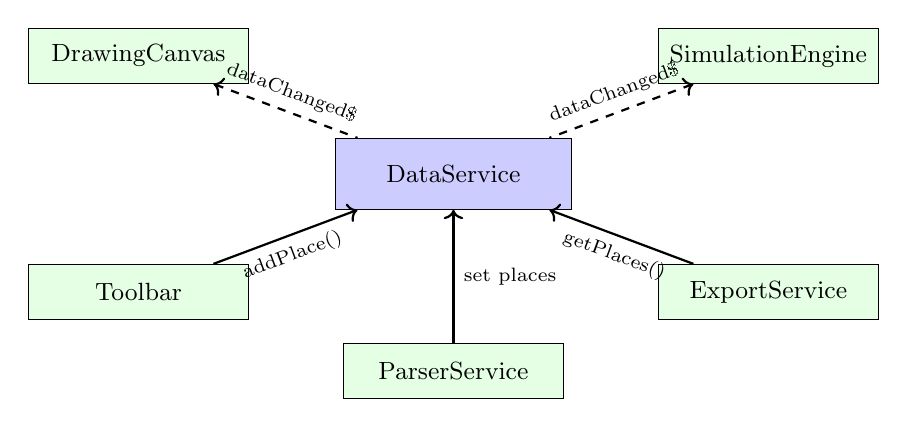
\begin{tikzpicture}[
        node distance=1.2cm,
        component/.style={rectangle, draw, fill=green!10, minimum width=2.8cm, minimum height=0.7cm, font=\small},
        service/.style={rectangle, draw, fill=blue!20, minimum width=3cm, minimum height=0.9cm, font=\small},
    ]
        % Central service
        \node[service] (ds) at (0,0) {DataService};
        
        % Components around it
        \node[component] (canvas) at (-4, 1.5) {DrawingCanvas};
        \node[component] (toolbar) at (-4, -1.5) {Toolbar};
        \node[component] (sim) at (4, 1.5) {SimulationEngine};
        \node[component] (export) at (4, -1.5) {ExportService};
        \node[component] (parser) at (0, -2.5) {ParserService};
        
        % Arrows
        \draw[->, thick] (toolbar) -- node[below, sloped, font=\scriptsize] {addPlace()} (ds);
        \draw[->, thick] (parser) -- node[right, font=\scriptsize] {set places} (ds);
        \draw[<-, thick, dashed] (canvas) -- node[above, sloped, font=\scriptsize] {dataChanged\$} (ds);
        \draw[<-, thick, dashed] (sim) -- node[above, sloped, font=\scriptsize] {dataChanged\$} (ds);
        \draw[->, thick] (export) -- node[below, sloped, font=\scriptsize] {getPlaces()} (ds);
        
    \end{tikzpicture}
    \caption{DataService as central hub for Petri net data}
    \label{fig:data-service-hub}
\end{figure}

The diagram shows:
\begin{itemize}
    \item \textbf{Solid arrows}: Components that \textit{modify} data (Toolbar adds elements, ParserService loads files)
    \item \textbf{Dashed arrows}: Components that \textit{subscribe} to changes (Canvas redraws, SimulationEngine recalculates)
    \item \textbf{Query arrows}: Components that \textit{read} data on demand (ExportService for saving)
\end{itemize}

\section{Interaction with Other Services}
\label{sec:data-interactions}

The \texttt{DataService} is used by nearly every other service:

\begin{table}[htb]
    \centering
    \begin{tabular}{ll}
        \toprule
        \textbf{Service} & \textbf{Interaction} \\
        \midrule
        \texttt{ParserService} & Loads data from JSON/PNML files \\
        \texttt{PnmlService} & Imports/exports PNML format \\
        \texttt{ExportJsonDataService} & Exports to custom JSON format \\
        \texttt{LayoutSugiyamaService} & Modifies element positions \\
        \texttt{ZoomService} & Reads element positions for bounds calculation \\
        \texttt{SimulationService} & Reads transitions for firing sequence \\
        \bottomrule
    \end{tabular}
    \caption{Services that interact with DataService}
    \label{tab:data-service-interactions}
\end{table}

\section{Summary}
\label{sec:data-summary}

The \texttt{DataService} is the application's \textbf{single source of truth} for Petri net data:

\begin{itemize}
    \item \textbf{Stores} all places, transitions, arcs, and actions
    \item \textbf{Provides} getter methods for reading current state
    \item \textbf{Offers} modification methods with automatic cascading (e.g., deleting connected arcs)
    \item \textbf{Broadcasts} changes via \texttt{dataChanged\$} observable
    \item \textbf{Enables} decoupled architecture where components don't directly communicate
\end{itemize}

With the core data model and storage understood, the next chapter explores how users interact with the canvas through \textbf{Zoom and Pan} functionality.


% Part III: System Design
\chapter{System Architecture}
\label{chap:architecture}

The previous chapters introduced the core building blocks: the \texttt{UiService} for managing UI state (Chapter~\ref{chap:ui-service}), the Petri net elements as data objects (Chapter~\ref{chap:petri-net-elements}), and the \texttt{DataService} as the central data store (Chapter~\ref{chap:data-service}). This chapter provides a high-level overview of how these components fit together within the overall system architecture.

\section{System Overview}
\label{sec:system-overview}

The L3S-Offshore-2 system follows a client-server architecture with clear separation between the visualization frontend and the simulation backend.

\begin{figure}[htb]
    \centering
    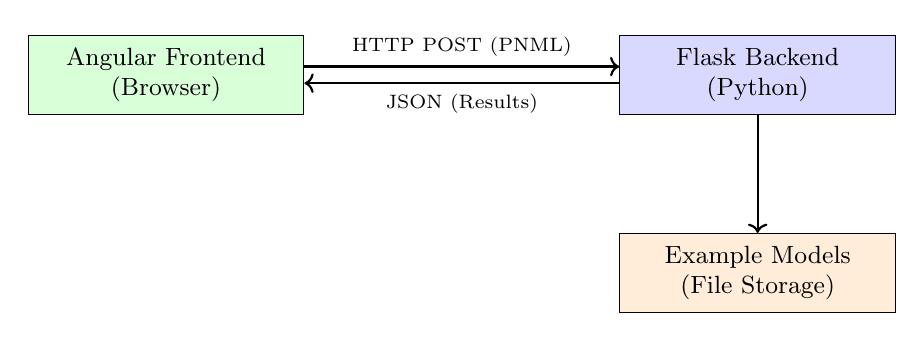
\begin{tikzpicture}[
        node distance=1.5cm,
        box/.style={rectangle, draw, minimum width=3.5cm, minimum height=1cm, align=center, font=\small},
        arrow/.style={->, thick},
    ]
        % Frontend
        \node[box, fill=green!15] (fe) {Angular Frontend\\(Browser)};
        
        % Backend
        \node[box, fill=blue!15, right=4cm of fe] (be) {Flask Backend\\(Python)};
        
        % Database/Storage
        \node[box, fill=orange!15, below=of be] (db) {Example Models\\(File Storage)};
        
        % Arrows
        \draw[arrow] ([yshift=3pt]fe.east) -- node[above, font=\scriptsize] {HTTP POST (PNML)} ([yshift=3pt]be.west);
        \draw[arrow] ([yshift=-3pt]be.west) -- node[below, font=\scriptsize] {JSON (Results)} ([yshift=-3pt]fe.east);
        \draw[arrow] (be) -- (db);
        
    \end{tikzpicture}
    \caption{High-level system architecture showing frontend-backend interaction}
    \label{fig:system-architecture}
\end{figure}

\subsection{Frontend (Angular)}

The frontend is a single-page application (SPA) responsible for:
\begin{itemize}
    \item Rendering Petri nets as interactive SVG graphics
    \item Handling user interactions (editing, navigation, simulation control)
    \item Managing application state across different tabs
    \item Communicating with the backend via REST API
\end{itemize}

\subsection{Backend (Flask)}

The Python backend provides:
\begin{itemize}
    \item PNML parsing and validation
    \item Petri net simulation using the \texttt{gspn4py} library
    \item Offshore scheduling algorithms
    \item Example model storage and retrieval
\end{itemize}

\section{Frontend Component Hierarchy}
\label{sec:component-hierarchy}

The Angular application is organized into a hierarchical component structure that reflects the UI layout.

\subsection{Root Components}

\begin{description}
    \item[AppComponent] The root component that bootstraps the application and contains the main layout
    \item[HeaderComponent] Displays the project banner with L3S branding
    \item[FooterComponent] Shows institutional logos with links to L3S and LUH homepages
\end{description}

\subsection{Tab Components}

The main content area uses Angular Material's tab group:

\begin{description}
    \item[ButtonBarComponent] The central coordinator that manages tab switching and toolbar rendering for each tab (Build, Code, Simulation, Analyze, Save, Offshore)
    \item[PetriNetComponent] Renders the interactive SVG visualization of the Petri net
    \item[CodeEditorComponent] Provides a text editor for direct PNML manipulation
    \item[ParameterTableComponent] Displays and edits simulation parameters
    \item[OffshoreViewComponent] Specialized view for offshore scheduling parameters
\end{description}

\subsection{Dialog Components}

Modal dialogs for user feedback and interaction:
\begin{description}
    \item[DataPersistenceInfoDialogComponent] Warns users about data loss on page reload
    \item[ErrorPopupComponent] Displays error messages from backend or parsing failures
    \item[HelpPopupComponent] Provides contextual help
    \item[TransitionFiringInfoPopupComponent] Shows firing statistics for transitions
\end{description}

\section{Service Layer}
\label{sec:service-layer}

Services are singleton classes that provide shared functionality and state management. The most important services are covered in dedicated chapters.

\subsection{Core Services}

\begin{description}
    \item[DataService] Central state container for the Petri net model. Manages places, transitions, arcs, and the current marking. Emits change events via RxJS observables. \textit{See Chapter~\ref{chap:data-service} for details.}
    
    \item[UiService] Manages UI state including the current tab, simulation mode (automatic/manual), selected elements, and zoom level. \textit{See Chapter~\ref{chap:ui-service} for details.}
    
    \item[ZoomService] Handles viewport transformations (pan, zoom) with ResizeObserver integration for responsive behavior. \textit{See Section~\ref{sec:zoom-pan-system} for details.}
    
    \item[ParserService] Converts between PNML XML, internal data structures, and the JSON representation used by the backend. \textit{See Chapter~\ref{chap:data-io} for details.}
\end{description}

\subsection{Simulation Services}

\begin{description}
    \item[SimulationService] Communicates with the backend's simulation endpoints. Manages firing sequences and multi-run results.
    
    \item[TokenGameService] Implements the manual simulation mode where users can step through the firing sequence or click on enabled transitions.
    
    \item[PlanningService] Handles the offshore scheduling API calls and parameter management. \textit{See Chapter~\ref{chap:planning-service} for details.}
\end{description}

\subsection{Utility Services}

\begin{description}
    \item[ExportImageService] Exports the current view as PNG
    \item[ExportSvgService] Exports the Petri net as SVG
    \item[ExportJsonDataService] Exports the internal representation as JSON. \textit{See Chapter~\ref{chap:data-io} for details.}
    \item[LayoutSugiyamaService] Implements the Sugiyama algorithm for automatic layout. \textit{See Chapter~\ref{chap:layout-algorithms} for details.}
\end{description}

\section{Data Flow}
\label{sec:data-flow}

\begin{figure}[htb]
    \centering
    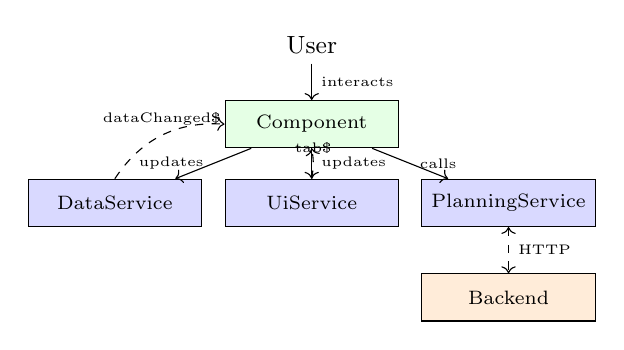
\begin{tikzpicture}[
        node distance=0.8cm,
        component/.style={rectangle, draw, fill=green!10, minimum width=2.2cm, minimum height=0.6cm, font=\scriptsize},
        service/.style={rectangle, draw, fill=blue!15, minimum width=2.2cm, minimum height=0.6cm, font=\scriptsize},
    ]
        % User
        \node (user) at (0, 2) {\small User};
        
        % Components
        \node[component] (comp) at (0, 1) {Component};
        
        % Services
        \node[service] (data) at (-2.5, 0) {DataService};
        \node[service] (ui) at (0, 0) {UiService};
        \node[service] (plan) at (2.5, 0) {PlanningService};
        
        % Backend
        \node[component, fill=orange!15] (back) at (2.5, -1.2) {Backend};
        
        % Arrows
        \draw[->] (user) -- node[right, font=\tiny] {interacts} (comp);
        \draw[->] (comp) -- node[left, font=\tiny] {updates} (data);
        \draw[->] (comp) -- node[right, font=\tiny] {updates} (ui);
        \draw[->] (comp) -- node[right, font=\tiny] {calls} (plan);
        \draw[<->, dashed] (plan) -- node[right, font=\tiny] {HTTP} (back);
        \draw[->, dashed] (data.north) to[bend left=30] node[above, font=\tiny] {dataChanged\$} (comp.west);
        \draw[->, dashed] (ui.north) to[bend right=10] node[above, font=\tiny] {tab\$} (comp.south);
        
    \end{tikzpicture}
    \caption{Data flow between components and services}
    \label{fig:data-flow}
\end{figure}

The application follows a unidirectional data flow pattern:

\begin{enumerate}
    \item \textbf{User Input:} User interacts with UI (clicks, drags, edits)
    \item \textbf{Component Handler:} Component method processes the event
    \item \textbf{Service Update:} Component calls service method to update state
    \item \textbf{Observable Emission:} Service emits new state via RxJS Subject
    \item \textbf{Subscriber Notification:} All subscribed components receive update
    \item \textbf{View Re-render:} Angular change detection updates the DOM
\end{enumerate}

\section{Tab State Management}
\label{sec:tab-state-management}

A key architectural feature is the tab-aware state management that ensures UI consistency when switching between tabs.

\subsection{The Tab\$ Observable}

The \texttt{UiService} exposes a \texttt{tab\$} BehaviorSubject that emits the current tab name whenever the user navigates:

\begin{lstlisting}[language=TypeScript, caption={Tab state observable in UiService}]
private _tab$ = new BehaviorSubject<string>('build');

get tab$(): Observable<string> {
  return this._tab$.asObservable();
}

set tab(value: string) {
  console.log(`[UiService] Tab changed: ${this._tab$.value} -> ${value}`);
  this._tab$.next(value);
}
\end{lstlisting}

\subsection{Tab Guards in Components}

Components subscribe to \texttt{tab\$} and conditionally enable/disable features:

\begin{lstlisting}[language=TypeScript, caption={Tab-aware highlighting in PetriNetComponent}]
this.uiService.tab$.subscribe(tab => {
  if (tab !== 'simulation') {
    this.clearAllHighlights();
    this.stopAnimationTimer();
  } else {
    this.restoreSimulationState();
  }
});
\end{lstlisting}


% Part IV: Implementation Details
\chapter{Implementation Details}
\label{chap:implementation}

This chapter describes the key implementation aspects of the frontend, focusing on the most complex and interesting technical solutions.

\section{Zoom and Pan System}
\label{sec:zoom-pan-system}

One of the most technically challenging aspects was implementing a robust zoom and pan system that behaves intuitively across different viewport sizes.

\subsection{The Problem}

The original fork had a basic zoom implementation that exhibited several issues:
\begin{itemize}
    \item Content would ``drift'' away from the center when zooming
    \item Mouse coordinates were incorrect after panning
    \item Elements would not be placed at the click position in the Build tab
    \item The ``Fit Content'' feature would not trigger correctly after loading a file
\end{itemize}

\subsection{Viewport-Centered Zooming}

The solution involved centering all zoom operations around the viewport center rather than the origin:

\begin{lstlisting}[language=TypeScript, caption={Viewport-centered zoom calculation}]
zoomAtCenter(factor: number): void {
  const viewportCenterX = this.viewportWidth / 2;
  const viewportCenterY = this.viewportHeight / 2;
  
  // Transform viewport center to SVG coordinates
  const svgX = (viewportCenterX - this.panX) / this.scale;
  const svgY = (viewportCenterY - this.panY) / this.scale;
  
  // Apply new scale
  this.scale *= factor;
  this.scale = Math.max(0.1, Math.min(5, this.scale));
  
  // Adjust pan to keep the same SVG point at viewport center
  this.panX = viewportCenterX - svgX * this.scale;
  this.panY = viewportCenterY - svgY * this.scale;
}
\end{lstlisting}

\subsection{ResizeObserver Integration}

To handle viewport size changes (e.g., when switching from the Code tab's 50\% width back to full width), a \texttt{ResizeObserver} was integrated:

\begin{lstlisting}[language=TypeScript, caption={ResizeObserver setup for responsive viewport}]
private resizeObserver: ResizeObserver;
private shouldAutoFit = false;

ngAfterViewInit(): void {
  this.resizeObserver = new ResizeObserver(entries => {
    for (const entry of entries) {
      this.zoomService.updateViewportDimensions(
        entry.contentRect.width,
        entry.contentRect.height
      );
      if (this.shouldAutoFit) {
        this.fitContentToViewport();
      }
    }
  });
  this.resizeObserver.observe(this.svgContainer.nativeElement);
}
\end{lstlisting}

\section{Simulation Animation}
\label{sec:simulation-animation}

The simulation animation system displays the firing sequence received from the backend.

\subsection{Firing Sequence Format}

The backend returns a firing sequence as an array of transition IDs:

\begin{lstlisting}[language=TypeScript, caption={Firing sequence data structure}]
interface SimulationResult {
  firing_seq: string[];      // e.g., ["t1", "t3", "t2", "t1"]
  detailed_log: StepLog[];   // Optional: token counts at each step
}
\end{lstlisting}

\subsection{Animation Loop}

The animation uses \texttt{setInterval} with a configurable speed:

\begin{lstlisting}[language=TypeScript, caption={Animation timer implementation}]
private animationTimer: any;

startAutoplay(): void {
  const interval = 1000 / this.playbackSpeed;
  this.animationTimer = setInterval(() => {
    if (this.currentStep < this.firingSequence.length) {
      this.highlightTransition(this.firingSequence[this.currentStep]);
      this.currentStep++;
      this.timelinePosition = this.currentStep;
    } else {
      this.stopAutoplay();
    }
  }, interval);
}
\end{lstlisting}

\subsection{Transition Highlighting}

Transitions are highlighted by applying CSS classes that trigger SVG animations:

\begin{lstlisting}[language=TypeScript, caption={Transition highlighting with CSS}]
highlightTransition(transitionId: string): void {
  // Remove previous highlight
  this.clearHighlights();
  
  // Find the SVG element
  const element = document.getElementById(`transition-${transitionId}`);
  if (element) {
    element.classList.add('firing');
    // CSS handles the animation:
    // .firing { fill: #ff6600; filter: drop-shadow(0 0 8px #ff6600); }
  }
}
\end{lstlisting}

\section{Token Reset Logic}
\label{sec:token-reset}

A critical feature is resetting tokens to the initial marking when leaving the Simulation tab.

\subsection{Baseline Snapshot}

When the user first enters the Simulation tab, a snapshot of the current marking is saved:

\begin{lstlisting}[language=TypeScript, caption={Baseline marking snapshot}]
private baselineMarking: Map<string, number> = new Map();

saveBaselineMarking(): void {
  this.dataService.places.forEach(place => {
    this.baselineMarking.set(place.id, place.tokens);
  });
}

resetTokensToBaseline(): void {
  this.baselineMarking.forEach((tokens, placeId) => {
    const place = this.dataService.getPlaceById(placeId);
    if (place) {
      place.tokens = tokens;
    }
  });
  this.dataService.triggerDataChanged();
}
\end{lstlisting}

\subsection{Tab-Aware Reset}

The reset is triggered when navigating away from the Simulation tab:

\begin{lstlisting}[language=TypeScript, caption={Tab-aware token reset}]
this.uiService.tab$.subscribe(newTab => {
  if (this.previousTab === 'simulation' && newTab !== 'simulation') {
    this.resetTokensToBaseline();
    this.clearAllHighlights();
  }
  if (newTab === 'simulation' && this.previousTab !== 'simulation') {
    this.saveBaselineMarking();
  }
  this.previousTab = newTab;
});
\end{lstlisting}

\section{Parameter Table}
\label{sec:parameter-table}

The parameter table allows users to configure simulation parameters before running.

\subsection{Dynamic Form Generation}

Parameters are dynamically generated from the backend's DTO definition:

\begin{lstlisting}[language=TypeScript, caption={Dynamic parameter form generation}]
generateFormControls(parameters: ParameterDefinition[]): void {
  parameters.forEach(param => {
    this.formGroup.addControl(
      param.name,
      new FormControl(param.defaultValue, this.getValidators(param))
    );
  });
}
\end{lstlisting}

\subsection{Reactive Forms Integration}

The initial implementation caused severe UI freezes due to incorrect parent-child form integration. The solution used Angular's \texttt{ControlContainer}:

\begin{lstlisting}[language=TypeScript, caption={ControlContainer fix for nested forms}]
@Component({
  selector: 'app-parameter-row',
  viewProviders: [
    { provide: ControlContainer, useExisting: FormGroupDirective }
  ]
})
export class ParameterRowComponent {
  // Child component now correctly integrates with parent form
}
\end{lstlisting}

\section{Right-Click Statistics}
\label{sec:right-click-statistics}

To avoid conflicts with the manual simulation mode (left-click fires transition), statistics are displayed via right-click.

\begin{lstlisting}[language=TypeScript, caption={Right-click handler for statistics popup}]
@HostListener('contextmenu', ['$event'])
onRightClick(event: MouseEvent): void {
  if (this.uiService.tab !== 'simulation') return;
  
  event.preventDefault(); // Suppress browser context menu
  
  const transitionId = this.getTransitionIdFromEvent(event);
  if (transitionId) {
    const stats = this.simulationService.getTransitionStats(transitionId);
    this.showStatisticsPopup(event.clientX, event.clientY, stats);
  }
}
\end{lstlisting}

\section{Data Persistence Warning}
\label{sec:data-persistence-warning}

Users are warned about data loss through two mechanisms:

\subsection{Initial Dialog}

A dialog appears on first visit (controlled by \texttt{localStorage}):

\begin{lstlisting}[language=TypeScript, caption={Data persistence dialog on app start}]
ngOnInit(): void {
  const shown = localStorage.getItem('dataPersistenceInfoShown');
  if (!shown) {
    this.dialog.open(DataPersistenceInfoDialogComponent);
  }
}
\end{lstlisting}

\subsection{Beforeunload Guard}

The browser's native confirmation dialog is triggered when closing with unsaved data:

\begin{lstlisting}[language=TypeScript, caption={Beforeunload event handler}]
@HostListener('window:beforeunload', ['$event'])
onBeforeUnload(event: BeforeUnloadEvent): void {
  if (!this.dataService.isEmpty()) {
    event.preventDefault();
    event.returnValue = ''; // Required for Chrome
  }
}
\end{lstlisting}

\chapter{PNML and JSON Data I/O}
\label{chap:data-io}

This chapter covers the application's data persistence capabilities: how Petri nets are saved to files and loaded from files. The I/O services act as translators between external file formats and the internal data structures.

\section{Problem Statement}
\label{sec:io-problem}

After spending time building a Petri net, users need to:
\begin{itemize}
    \item \textbf{Save} their work for later continuation
    \item \textbf{Share} models with colleagues
    \item \textbf{Load} existing models from other tools
\end{itemize}

Without I/O capabilities, all work would be lost when closing the browser. The application supports two file formats to address different needs.

\section{Supported Formats}
\label{sec:io-formats}

\begin{table}[htb]
    \centering
    \begin{tabular}{lll}
        \toprule
        \textbf{Feature} & \textbf{PNML} & \textbf{Custom JSON} \\
        \midrule
        Format type & XML-based & JSON \\
        Standard & ISO/IEC 15909-2 & Application-specific \\
        Complexity & Verbose, detailed & Concise, simple \\
        Interoperability & WoPeD, CPN Tools, etc. & This application only \\
        Human-readable & Moderate & High \\
        \bottomrule
    \end{tabular}
    \caption{Comparison of supported file formats}
    \label{tab:format-comparison}
\end{table}

\section{Custom JSON Format}
\label{sec:json-format}

The custom JSON format is designed for simplicity and ease of parsing:

\begin{lstlisting}[language=TypeScript, caption={JSON format interface (src/app/classes/json-petri-net.ts)}]
/**
 * Structure of our custom JSON format for Petri nets.
 */
export interface JsonPetriNet {
    /** List of place IDs, e.g., ["p1", "p2", "p3"] */
    places: string[];
    
    /** List of transition IDs, e.g., ["t1", "t2"] */
    transitions: string[];
    
    /** Arc definitions as "source,target": weight pairs */
    arcs?: { [idPair: string]: number };  // e.g., "p1,t1": 1
    
    /** Unique action labels for transitions */
    actions?: string[];
    
    /** Transition labels as id: label pairs */
    labels?: { [transitionId: string]: string };
    
    /** Initial marking as id: tokenCount pairs */
    marking?: { [placeId: string]: number };
    
    /** Element positions as id: {x, y} pairs */
    layout?: { [id: string]: Coords | Coords[] };
}

export interface Coords {
    x: number;
    y: number;
}
\end{lstlisting}

\subsection{Example JSON File}

\begin{lstlisting}[language=json, caption={Example Petri net in JSON format}]
{
  "places": ["p1", "p2", "p3"],
  "transitions": ["t1", "t2"],
  "arcs": {
    "p1,t1": 1,
    "t1,p2": 1,
    "p2,t2": 1,
    "t2,p3": 1
  },
  "marking": {
    "p1": 1,
    "p2": 0,
    "p3": 0
  },
  "labels": {
    "t1": "Stamp Letter",
    "t2": "Mail Letter"
  },
  "layout": {
    "p1": {"x": 100, "y": 100},
    "t1": {"x": 200, "y": 100},
    "p2": {"x": 300, "y": 100},
    "t2": {"x": 400, "y": 100},
    "p3": {"x": 500, "y": 100}
  }
}
\end{lstlisting}

\section{Exporting to JSON}
\label{sec:json-export}

The \texttt{ExportJsonDataService} converts the internal data model to JSON format:

\begin{lstlisting}[language=TypeScript, caption={JSON export service (src/app/tr-services/export-json-data.service.ts)}]
import { Injectable } from '@angular/core';
import { DataService } from './data.service';
import { JsonPetriNet, Coords } from '../classes/json-petri-net';

@Injectable({ providedIn: 'root' })
export class ExportJsonDataService {
    constructor(private dataService: DataService) {}

    /**
     * Export the current Petri net as a JSON file download.
     */
    public exportAsJson(): void {
        // 1. Build the JsonPetriNet structure
        const jsonObj = this.buildJsonStructure();
        
        // 2. Serialize to formatted JSON string
        const jsonString = JSON.stringify(jsonObj, null, 2);
        
        // 3. Trigger browser download
        this.downloadFile(jsonString, 'petri-net.json', 'application/json');
    }

    private buildJsonStructure(): JsonPetriNet {
        const json: JsonPetriNet = {
            places: [],
            transitions: [],
            arcs: {},
            marking: {},
            labels: {},
            layout: {},
        };

        // Collect places
        for (const place of this.dataService.getPlaces()) {
            json.places.push(place.id);
            json.layout![place.id] = { x: place.position.x, y: place.position.y };
            
            if (place.token > 0) {
                json.marking![place.id] = place.token;
            }
        }

        // Collect transitions
        for (const transition of this.dataService.getTransitions()) {
            json.transitions.push(transition.id);
            json.layout![transition.id] = { 
                x: transition.position.x, 
                y: transition.position.y 
            };
            
            if (transition.label) {
                json.labels![transition.id] = transition.label;
            }
        }

        // Collect arcs
        for (const arc of this.dataService.getArcs()) {
            const key = `${arc.from.id},${arc.to.id}`;
            json.arcs![key] = arc.weight;
            
            // Store anchor points if present
            if (arc.anchors.length > 0) {
                json.layout![key] = arc.anchors.map(p => ({ x: p.x, y: p.y }));
            }
        }

        return json;
    }

    private downloadFile(content: string, filename: string, mimeType: string): void {
        const blob = new Blob([content], { type: mimeType });
        const url = URL.createObjectURL(blob);
        
        const link = document.createElement('a');
        link.href = url;
        link.download = filename;
        link.click();
        
        URL.revokeObjectURL(url);
    }
}
\end{lstlisting}

\section{Importing from JSON}
\label{sec:json-import}

The \texttt{ParserService} converts JSON files back to internal objects:

\begin{lstlisting}[language=TypeScript, caption={JSON parser service (src/app/tr-services/parser.service.ts)}]
import { Injectable } from '@angular/core';
import { JsonPetriNet, Coords } from '../classes/json-petri-net';
import { Place } from '../tr-classes/petri-net/place';
import { Transition } from '../tr-classes/petri-net/transition';
import { Arc } from '../tr-classes/petri-net/arc';
import { Point } from '../tr-classes/petri-net/point';

@Injectable({ providedIn: 'root' })
export class ParserService {
    /** Flag: true if some elements had no position data */
    incompleteLayoutData: boolean = false;

    /**
     * Parse a JSON string into Petri net elements.
     * Returns arrays of places, transitions, arcs, and actions.
     */
    parse(jsonText: string): [Place[], Transition[], Arc[], string[]] {
        this.incompleteLayoutData = false;
        
        // 1. Parse JSON string to object
        const data: JsonPetriNet = JSON.parse(jsonText);
        
        const places: Place[] = [];
        const transitions: Transition[] = [];
        const arcs: Arc[] = [];
        const actions: string[] = data.actions || [];

        // 2. Create Place objects
        for (const placeId of data.places) {
            const position = this.getPosition(data, placeId);
            const tokens = data.marking?.[placeId] || 0;
            const label = data.labels?.[placeId];
            
            places.push(new Place(tokens, position, placeId, label));
        }

        // 3. Create Transition objects
        for (const transitionId of data.transitions) {
            const position = this.getPosition(data, transitionId);
            const label = data.labels?.[transitionId];
            
            transitions.push(new Transition(position, transitionId, label));
        }

        // 4. Create Arc objects and link to nodes
        if (data.arcs) {
            for (const [idPair, weight] of Object.entries(data.arcs)) {
                const [fromId, toId] = idPair.split(',');
                
                const fromNode = this.findNode(fromId, places, transitions);
                const toNode = this.findNode(toId, places, transitions);
                
                if (fromNode && toNode) {
                    const anchors = this.getAnchors(data, idPair);
                    const arc = new Arc(fromNode, toNode, weight, anchors);
                    arcs.push(arc);
                    
                    // Register with transition
                    if (toNode instanceof Transition) {
                        toNode.appendPreArc(arc);
                    }
                    if (fromNode instanceof Transition) {
                        fromNode.appendPostArc(arc);
                    }
                }
            }
        }

        return [places, transitions, arcs, actions];
    }

    /**
     * Get position from layout data, or return default (0,0).
     */
    private getPosition(data: JsonPetriNet, id: string): Point {
        if (data.layout && data.layout[id]) {
            const coords = data.layout[id] as Coords;
            return new Point(coords.x, coords.y);
        }
        
        this.incompleteLayoutData = true;
        return new Point(0, 0);
    }

    /**
     * Get arc anchor points from layout data.
     */
    private getAnchors(data: JsonPetriNet, arcId: string): Point[] {
        if (data.layout && Array.isArray(data.layout[arcId])) {
            return (data.layout[arcId] as Coords[]).map(c => new Point(c.x, c.y));
        }
        return [];
    }

    /**
     * Find a node (place or transition) by ID.
     */
    private findNode(id: string, places: Place[], transitions: Transition[]): Place | Transition | undefined {
        return places.find(p => p.id === id) || transitions.find(t => t.id === id);
    }
}
\end{lstlisting}

\section{PNML Format}
\label{sec:pnml-format}

PNML (Petri Net Markup Language) is an XML-based international standard:

\begin{lstlisting}[language=XML, caption={Example PNML document structure}]
<?xml version="1.0" encoding="UTF-8"?>
<pnml>
  <net id="net1" type="http://www.pnml.org/version-2009/grammar/ptnet">
    <page id="page1">
      <place id="p1">
        <name><text>Unstamped Letter</text></name>
        <graphics>
          <position x="100" y="100"/>
        </graphics>
        <initialMarking>
          <text>1</text>
        </initialMarking>
      </place>
      
      <transition id="t1">
        <name><text>Stamp Letter</text></name>
        <graphics>
          <position x="200" y="100"/>
        </graphics>
      </transition>
      
      <arc id="a1" source="p1" target="t1">
        <inscription><text>1</text></inscription>
      </arc>
    </page>
  </net>
</pnml>
\end{lstlisting}

\section{PNML Import and Export}
\label{sec:pnml-service}

The \texttt{PnmlService} handles bidirectional PNML conversion:

\begin{lstlisting}[language=TypeScript, caption={PNML service (src/app/tr-services/pnml.service.ts) - Import}]
import { Injectable } from '@angular/core';
import { xml2js } from 'xml-js';
import { DataService } from './data.service';
import { Place } from '../tr-classes/petri-net/place';
import { Transition } from '../tr-classes/petri-net/transition';
import { Arc } from '../tr-classes/petri-net/arc';
import { Point } from '../tr-classes/petri-net/point';

@Injectable({ providedIn: 'root' })
export class PnmlService {
    incompleteLayoutData: boolean = false;

    constructor(
        private dataService: DataService,
        private layoutService: LayoutSugiyamaService
    ) {}

    /**
     * Parse PNML XML string and load into DataService.
     */
    parse(xmlString: string): [Place[], Transition[], Arc[], string[]] {
        this.incompleteLayoutData = false;
        
        // 1. Convert XML to JavaScript object
        const xmlObj = xml2js(xmlString, { compact: false });
        
        // 2. Find all place, transition, and arc elements
        const pnmlPlaces = this.findElements(xmlObj, 'place');
        const pnmlTransitions = this.findElements(xmlObj, 'transition');
        const pnmlArcs = this.findElements(xmlObj, 'arc');
        
        // 3. Convert to internal objects
        const places = this.parsePlaces(pnmlPlaces);
        const transitions = this.parseTransitions(pnmlTransitions);
        const arcs = this.parseArcs(pnmlArcs, places, transitions);
        const actions = this.extractActions(transitions);
        
        // 4. Update DataService
        this.dataService.places = places;
        this.dataService.transitions = transitions;
        this.dataService.arcs = arcs;
        this.dataService.actions = actions;
        
        // 5. Apply automatic layout if positions were missing
        if (this.incompleteLayoutData) {
            this.layoutService.applySugiyamaLayout();
        }
        
        this.dataService.triggerDataChanged(true);
        
        return [places, transitions, arcs, actions];
    }

    /**
     * Parse a PNML place element into a Place object.
     */
    private parsePlace(element: any): Place {
        const id = element.attributes.id;
        
        // Extract name from nested <name><text> elements
        const nameElement = this.findChild(element, 'name');
        const label = nameElement ? this.getTextContent(nameElement) : undefined;
        
        // Extract position from <graphics><position>
        const position = this.extractPosition(element);
        
        // Extract initial marking from <initialMarking><text>
        const markingElement = this.findChild(element, 'initialMarking');
        const tokens = markingElement ? parseInt(this.getTextContent(markingElement)) || 0 : 0;
        
        return new Place(tokens, position, id, label);
    }

    /**
     * Extract position from graphics element, or mark as incomplete.
     */
    private extractPosition(element: any): Point {
        const graphics = this.findChild(element, 'graphics');
        const position = graphics ? this.findChild(graphics, 'position') : null;
        
        if (position?.attributes?.x && position?.attributes?.y) {
            return new Point(
                parseFloat(position.attributes.x),
                parseFloat(position.attributes.y)
            );
        }
        
        this.incompleteLayoutData = true;
        return new Point(0, 0);
    }
    
    // ... additional helper methods ...
}
\end{lstlisting}

\subsection{PNML Export}

\begin{lstlisting}[language=TypeScript, caption={PNML export method}]
/**
 * Generate PNML XML string from current DataService content.
 */
public getPNML(): string {
    const places = this.dataService.getPlaces();
    const transitions = this.dataService.getTransitions();
    const arcs = this.dataService.getArcs();
    
    // Build XML structure
    let xml = `<?xml version="1.0" encoding="UTF-8"?>
<pnml>
  <net id="net1" type="http://www.pnml.org/version-2009/grammar/ptnet">
    <page id="page1">
`;
    
    // Add places
    for (const place of places) {
        xml += this.placeToXml(place);
    }
    
    // Add transitions
    for (const transition of transitions) {
        xml += this.transitionToXml(transition);
    }
    
    // Add arcs
    for (const arc of arcs) {
        xml += this.arcToXml(arc);
    }
    
    xml += `    </page>
  </net>
</pnml>`;
    
    return this.formatXml(xml);
}

private placeToXml(place: Place): string {
    return `      <place id="${place.id}">
        <name><text>${place.label || ''}</text></name>
        <graphics>
          <position x="${place.position.x}" y="${place.position.y}"/>
        </graphics>
        <initialMarking><text>${place.token}</text></initialMarking>
      </place>
`;
}

private transitionToXml(transition: Transition): string {
    return `      <transition id="${transition.id}">
        <name><text>${transition.label || ''}</text></name>
        <graphics>
          <position x="${transition.position.x}" y="${transition.position.y}"/>
        </graphics>
      </transition>
`;
}

private arcToXml(arc: Arc): string {
    return `      <arc id="arc-${arc.from.id}-${arc.to.id}" source="${arc.from.id}" target="${arc.to.id}">
        <inscription><text>${arc.weight}</text></inscription>
      </arc>
`;
}
\end{lstlisting}

\section{Import Flow Visualization}
\label{sec:io-flow}

\begin{figure}[htb]
    \centering
    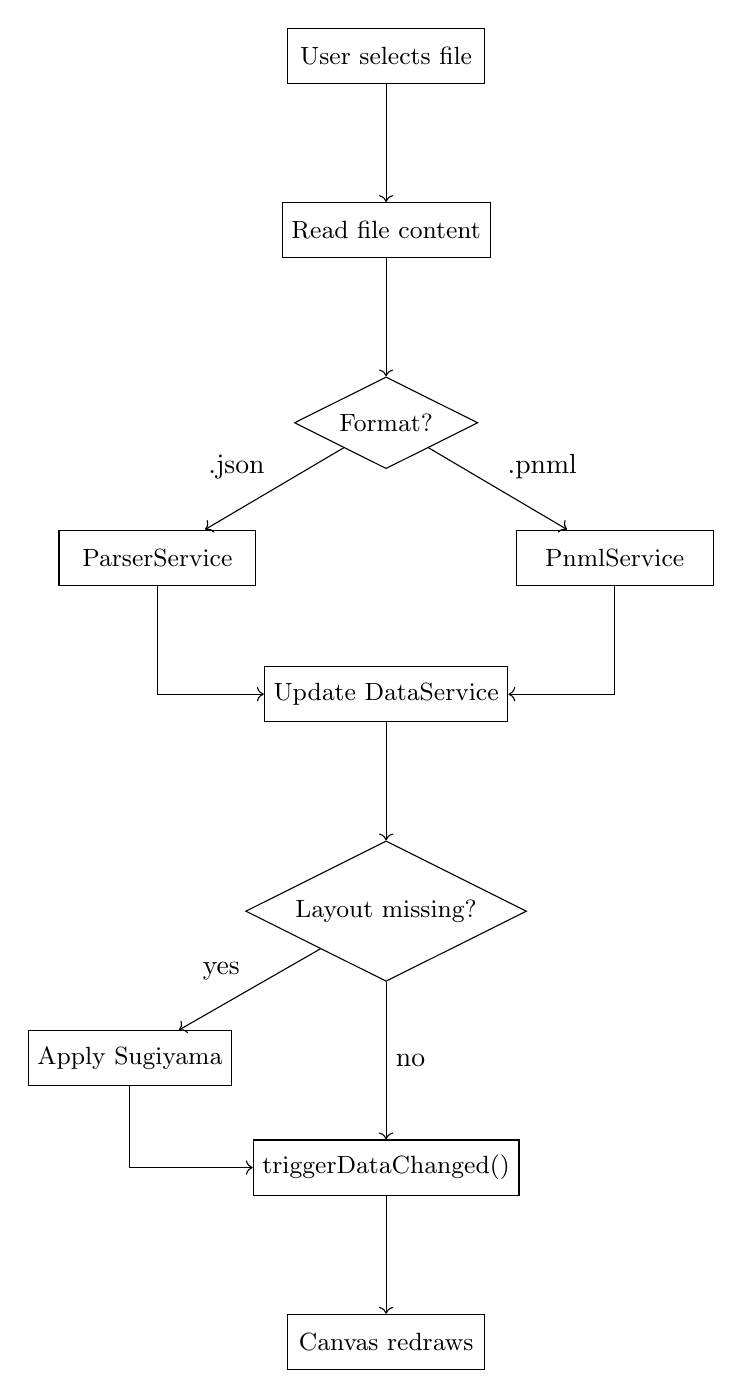
\begin{tikzpicture}[
        node distance=1.5cm,
        box/.style={rectangle, draw, minimum width=2.5cm, minimum height=0.7cm, font=\small},
        decision/.style={diamond, draw, aspect=2, font=\small},
    ]
        \node[box] (file) {User selects file};
        \node[box, below=of file] (read) {Read file content};
        \node[decision, below=of read] (format) {Format?};
        \node[box, below left=of format] (json) {ParserService};
        \node[box, below right=of format] (pnml) {PnmlService};
        \node[box, below=2.5cm of format] (data) {Update DataService};
        \node[decision, below=of data] (layout) {Layout missing?};
        \node[box, below left=of layout] (sugiyama) {Apply Sugiyama};
        \node[box, below=2cm of layout] (notify) {triggerDataChanged()};
        \node[box, below=of notify] (redraw) {Canvas redraws};
        
        \draw[->] (file) -- (read);
        \draw[->] (read) -- (format);
        \draw[->] (format) -- node[above left] {.json} (json);
        \draw[->] (format) -- node[above right] {.pnml} (pnml);
        \draw[->] (json) |- (data);
        \draw[->] (pnml) |- (data);
        \draw[->] (data) -- (layout);
        \draw[->] (layout) -- node[above left] {yes} (sugiyama);
        \draw[->] (layout) -- node[right] {no} (notify);
        \draw[->] (sugiyama) |- (notify);
        \draw[->] (notify) -- (redraw);
    \end{tikzpicture}
    \caption{File import processing flow}
    \label{fig:import-flow}
\end{figure}

\section{Handling Missing Layout Data}
\label{sec:missing-layout}

When loading files without position information (common with PNML files from other tools), the services set \texttt{incompleteLayoutData = true}. The calling code then automatically applies the Sugiyama layout algorithm (covered in the next chapter) to generate readable positions.

\section{Summary}
\label{sec:io-summary}

The I/O services enable data persistence and interoperability:

\begin{itemize}
    \item \textbf{ExportJsonDataService}: Exports to custom JSON format
    \item \textbf{ParserService}: Imports from custom JSON format
    \item \textbf{PnmlService}: Bidirectional PNML (XML) conversion
    \item \textbf{Automatic layout}: Applied when position data is missing
    \item \textbf{Download trigger}: Browser's download API for file saving
\end{itemize}

The next chapter covers the \textbf{Layout Algorithms} that automatically arrange Petri net elements into readable configurations.

\chapter{Layout Algorithms}
\label{chap:layout-algorithms}

When loading a Petri net without position information, or after extensive manual editing, the diagram can become cluttered and difficult to read. This chapter covers the automatic layout algorithms that transform messy diagrams into clear, structured visualizations.

\section{Problem Statement}
\label{sec:layout-problem}

Consider importing a PNML file from another tool that stored no graphical information. All elements would be placed at position $(0, 0)$, creating an unusable overlap. Even with positions, diagrams can suffer from:

\begin{itemize}
    \item \textbf{Overlapping elements}: Places and transitions stacked on each other
    \item \textbf{Arc crossings}: Lines crossing unnecessarily, obscuring the flow
    \item \textbf{Poor spacing}: Elements too close or too far apart
    \item \textbf{No visual hierarchy}: The logical flow of the process is not apparent
\end{itemize}

Layout algorithms solve these problems by calculating optimal positions for all elements.

\section{Available Algorithms}
\label{sec:layout-algorithms}

The application provides two layout algorithms with different characteristics:

\begin{table}[htb]
    \centering
    \begin{tabular}{lll}
        \toprule
        \textbf{Algorithm} & \textbf{Approach} & \textbf{Best For} \\
        \midrule
        Spring Embedder & Physics simulation & General, organic layouts \\
        Sugiyama & Hierarchical layering & Sequential processes, flowcharts \\
        \bottomrule
    \end{tabular}
    \caption{Layout algorithm comparison}
    \label{tab:layout-comparison}
\end{table}

\section{Spring Embedder Algorithm}
\label{sec:spring-embedder}

The Spring Embedder models the Petri net as a physical system:

\begin{itemize}
    \item \textbf{Nodes} act as electrically charged particles that \textbf{repel} each other
    \item \textbf{Arcs} act as springs that \textbf{attract} connected nodes toward an ideal length
\end{itemize}

The algorithm iteratively moves nodes until forces reach equilibrium.

\subsection{Force Calculation}

For each node, the total force is the sum of:
\begin{enumerate}
    \item \textbf{Repulsion} from all other nodes: $F_{rep} = \frac{C_{rep}}{d^2}$
    \item \textbf{Spring attraction/repulsion} from connected nodes: $F_{spring} = C_{spring} \cdot (d - L)$
\end{enumerate}

Where $d$ is the distance between nodes, $L$ is the ideal arc length, and $C_{rep}$, $C_{spring}$ are constants.

\begin{lstlisting}[language=TypeScript, caption={Spring Embedder implementation (src/app/tr-services/layout-spring-embedder.service.ts)}]
import { Injectable } from '@angular/core';
import { DataService } from './data.service';
import { Point } from '../tr-classes/petri-net/point';
import { Node } from '../tr-interfaces/petri-net/node';

@Injectable({ providedIn: 'root' })
export class LayoutSpringEmbedderService {
    // Algorithm parameters
    private epsilon = 0.01;       // Minimum force for termination
    private maxIterations = 5000; // Maximum iteration count
    private cRep = 20000;         // Repulsion constant
    private idealLength = 150;    // Ideal arc length
    private cSpring = 20;         // Spring constant

    constructor(private dataService: DataService) {}

    /**
     * Apply Spring Embedder layout to all nodes.
     * Runs asynchronously with visual feedback.
     */
    async layoutSpringEmbedder(): Promise<void> {
        const nodes: Node[] = [
            ...this.dataService.getPlaces(),
            ...this.dataService.getTransitions()
        ];

        // Initialize random positions if all at origin
        this.initializePositions(nodes);

        let maxForce = this.epsilon + 1;
        let iteration = 0;

        // Iterate until equilibrium or max iterations
        while (iteration < this.maxIterations && maxForce > this.epsilon) {
            const forces: Map<string, Point> = new Map();

            // Calculate forces for each node
            for (const node of nodes) {
                const force = this.calculateTotalForce(node, nodes);
                forces.set(node.id, force);
            }

            // Apply forces and track maximum
            maxForce = 0;
            for (const node of nodes) {
                const force = forces.get(node.id)!;
                node.position.x += force.x;
                node.position.y += force.y;

                const magnitude = Math.sqrt(force.x ** 2 + force.y ** 2);
                maxForce = Math.max(maxForce, magnitude);
            }

            // Yield for UI updates (every 10 iterations)
            if (iteration % 10 === 0) {
                this.dataService.triggerDataChanged();
                await this.sleep(1);
            }

            iteration++;
        }

        console.log(`Spring Embedder completed in ${iteration} iterations`);
        this.dataService.triggerDataChanged(true);
    }

    /**
     * Calculate total force on a node from all other nodes.
     */
    private calculateTotalForce(node: Node, allNodes: Node[]): Point {
        let fx = 0, fy = 0;

        for (const other of allNodes) {
            if (other.id === node.id) continue;

            // Repulsion force (always present)
            const repulsion = this.calculateRepulsion(node.position, other.position);
            fx += repulsion.x;
            fy += repulsion.y;

            // Spring force (only for connected nodes)
            if (this.areConnected(node, other)) {
                const spring = this.calculateSpring(node.position, other.position);
                fx += spring.x;
                fy += spring.y;
            }
        }

        return new Point(fx, fy);
    }

    /**
     * Calculate repulsion force between two positions.
     * Inversely proportional to distance squared.
     */
    private calculateRepulsion(p1: Point, p2: Point): Point {
        const dx = p1.x - p2.x;
        const dy = p1.y - p2.y;
        const distance = Math.sqrt(dx * dx + dy * dy);

        // Prevent division by zero
        if (distance < 0.1) {
            return new Point(
                (Math.random() - 0.5) * 10,
                (Math.random() - 0.5) * 10
            );
        }

        const factor = this.cRep / (distance * distance);
        return new Point(
            (dx / distance) * factor,
            (dy / distance) * factor
        );
    }

    /**
     * Calculate spring force between connected nodes.
     * Attracts if too far, repels if too close.
     */
    private calculateSpring(p1: Point, p2: Point): Point {
        const dx = p2.x - p1.x;
        const dy = p2.y - p1.y;
        const distance = Math.sqrt(dx * dx + dy * dy);

        if (distance < 0.1) return new Point(0, 0);

        // Displacement from ideal length
        const displacement = distance - this.idealLength;
        const factor = this.cSpring * displacement / distance;

        return new Point(dx * factor, dy * factor);
    }

    private sleep(ms: number): Promise<void> {
        return new Promise(resolve => setTimeout(resolve, ms));
    }

    // ... helper methods ...
}
\end{lstlisting}

\section{Sugiyama Algorithm}
\label{sec:sugiyama}

The Sugiyama algorithm~\cite{Sugiyama1981} creates hierarchical, layered layouts ideal for sequential processes. It operates in four phases:

\begin{enumerate}
    \item \textbf{Cycle Removal}: Temporarily reverse some arcs to create a DAG
    \item \textbf{Layer Assignment}: Assign nodes to horizontal layers
    \item \textbf{Vertex Ordering}: Order nodes within layers to minimize crossings
    \item \textbf{Coordinate Assignment}: Calculate final x, y positions
\end{enumerate}

\subsection{Phase 1: Cycle Removal}

Petri nets often contain cycles (feedback loops). For hierarchical layout, cycles must be temporarily broken:

\begin{lstlisting}[language=TypeScript, caption={Cycle removal service}]
export class CycleRemovalService {
    private reversedArcs: Arc[] = [];

    constructor(private nodes: Node[], private arcs: Arc[]) {}

    /**
     * Remove cycles by reversing back-edges.
     * Uses depth-first search to detect cycles.
     */
    removeCycles(): void {
        const visited = new Set<string>();
        const recursionStack = new Set<string>();

        for (const node of this.nodes) {
            if (!visited.has(node.id)) {
                this.dfs(node, visited, recursionStack);
            }
        }
    }

    private dfs(node: Node, visited: Set<string>, stack: Set<string>): void {
        visited.add(node.id);
        stack.add(node.id);

        const outgoingArcs = this.arcs.filter(a => a.from.id === node.id);
        
        for (const arc of outgoingArcs) {
            const targetId = arc.to.id;
            
            if (stack.has(targetId)) {
                // Back-edge detected: reverse this arc
                this.reverseArc(arc);
                this.reversedArcs.push(arc);
            } else if (!visited.has(targetId)) {
                this.dfs(arc.to, visited, stack);
            }
        }

        stack.delete(node.id);
    }

    /**
     * Restore reversed arcs after layout is complete.
     */
    reverseArcs(): void {
        for (const arc of this.reversedArcs) {
            this.reverseArc(arc);
        }
    }

    private reverseArc(arc: Arc): void {
        const temp = arc.from;
        arc.from = arc.to;
        arc.to = temp;
    }
}
\end{lstlisting}

\subsection{Phase 2: Layer Assignment}

Nodes are assigned to layers based on their distance from source nodes:

\begin{lstlisting}[language=TypeScript, caption={Layer assignment service}]
export class LayerAssignmentService {
    constructor(private nodes: Node[], private arcs: Arc[]) {}

    /**
     * Assign each node to a layer using longest-path algorithm.
     * Returns array of layers, each containing nodes at that level.
     */
    assignLayers(): Node[][] {
        const layers: Node[][] = [];
        const nodeLayer = new Map<string, number>();

        // Find source nodes (no incoming arcs)
        const sources = this.nodes.filter(n => 
            !this.arcs.some(a => a.to.id === n.id)
        );

        // Assign sources to layer 0
        for (const source of sources) {
            nodeLayer.set(source.id, 0);
        }

        // BFS to assign remaining nodes
        const queue = [...sources];
        while (queue.length > 0) {
            const node = queue.shift()!;
            const currentLayer = nodeLayer.get(node.id)!;

            // Find successors
            const outArcs = this.arcs.filter(a => a.from.id === node.id);
            for (const arc of outArcs) {
                const successor = arc.to;
                const newLayer = currentLayer + 1;

                // Update if this path is longer
                if (!nodeLayer.has(successor.id) || 
                    nodeLayer.get(successor.id)! < newLayer) {
                    nodeLayer.set(successor.id, newLayer);
                    queue.push(successor);
                }
            }
        }

        // Build layer arrays
        const maxLayer = Math.max(...nodeLayer.values());
        for (let i = 0; i <= maxLayer; i++) {
            layers[i] = this.nodes.filter(n => nodeLayer.get(n.id) === i);
        }

        return layers;
    }
}
\end{lstlisting}

\subsection{Phase 3: Vertex Ordering}

Within each layer, nodes are reordered to minimize arc crossings:

\begin{lstlisting}[language=TypeScript, caption={Vertex ordering (barycenter method)}]
export class VertexOrderingService {
    constructor(
        private layers: Node[][],
        private arcs: Arc[]
    ) {}

    /**
     * Order vertices using barycenter heuristic.
     * Minimizes edge crossings between adjacent layers.
     */
    orderVertices(): void {
        // Multiple passes for better results
        for (let pass = 0; pass < 4; pass++) {
            // Forward pass
            for (let i = 1; i < this.layers.length; i++) {
                this.orderLayer(i, i - 1);
            }
            // Backward pass
            for (let i = this.layers.length - 2; i >= 0; i--) {
                this.orderLayer(i, i + 1);
            }
        }
    }

    /**
     * Order nodes in targetLayer based on connections to fixedLayer.
     */
    private orderLayer(targetIdx: number, fixedIdx: number): void {
        const targetLayer = this.layers[targetIdx];
        const fixedLayer = this.layers[fixedIdx];

        // Calculate barycenter for each node
        const barycenters = targetLayer.map(node => {
            const connectedIndices = this.getConnectedIndices(node, fixedLayer);
            if (connectedIndices.length === 0) return Infinity;
            
            const sum = connectedIndices.reduce((a, b) => a + b, 0);
            return sum / connectedIndices.length;
        });

        // Sort by barycenter
        const indexed = targetLayer.map((node, i) => ({ node, bc: barycenters[i] }));
        indexed.sort((a, b) => a.bc - b.bc);
        
        this.layers[targetIdx] = indexed.map(item => item.node);
    }

    private getConnectedIndices(node: Node, layer: Node[]): number[] {
        const indices: number[] = [];
        
        for (const arc of this.arcs) {
            let connected: Node | null = null;
            if (arc.from.id === node.id) connected = arc.to;
            if (arc.to.id === node.id) connected = arc.from;
            
            if (connected) {
                const idx = layer.findIndex(n => n.id === connected!.id);
                if (idx !== -1) indices.push(idx);
            }
        }
        
        return indices;
    }
}
\end{lstlisting}

\subsection{Phase 4: Coordinate Assignment}

Finally, x and y coordinates are calculated based on layers and ordering:

\begin{lstlisting}[language=TypeScript, caption={Coordinate assignment}]
export class CoordinateAssignmentService {
    private layerSpacing = 180;  // Horizontal space between layers
    private nodeSpacing = 100;   // Vertical space between nodes

    constructor(
        private layers: Node[][],
        private canvasWidth: number = 1200,
        private canvasHeight: number = 600
    ) {}

    /**
     * Assign final coordinates to all nodes.
     */
    assignCoordinates(): void {
        const totalWidth = (this.layers.length - 1) * this.layerSpacing;
        const startX = (this.canvasWidth - totalWidth) / 2;

        for (let layerIdx = 0; layerIdx < this.layers.length; layerIdx++) {
            const layer = this.layers[layerIdx];
            const x = startX + layerIdx * this.layerSpacing;

            // Center nodes vertically
            const totalHeight = (layer.length - 1) * this.nodeSpacing;
            const startY = (this.canvasHeight - totalHeight) / 2;

            for (let nodeIdx = 0; nodeIdx < layer.length; nodeIdx++) {
                const node = layer[nodeIdx];
                const y = startY + nodeIdx * this.nodeSpacing;
                
                node.position = new Point(x, y);
            }
        }
    }
}
\end{lstlisting}

\subsection{Orchestrating the Phases}

\begin{lstlisting}[language=TypeScript, caption={Sugiyama layout service (src/app/tr-services/layout-sugiyama.service.ts)}]
@Injectable({ providedIn: 'root' })
export class LayoutSugiyamaService {
    constructor(private dataService: DataService) {}

    /**
     * Apply complete Sugiyama layout algorithm.
     */
    applySugiyamaLayout(): void {
        const nodes = [
            ...this.dataService.getPlaces(),
            ...this.dataService.getTransitions()
        ];
        const arcs = [...this.dataService.getArcs()];

        // Phase 1: Remove cycles
        const cycleRemoval = new CycleRemovalService(nodes, arcs);
        cycleRemoval.removeCycles();

        // Phase 2: Assign layers
        const layerAssignment = new LayerAssignmentService(nodes, arcs);
        const layers = layerAssignment.assignLayers();

        // Restore original arc directions
        cycleRemoval.reverseArcs();

        // Phase 3: Order vertices
        const vertexOrdering = new VertexOrderingService(layers, arcs);
        vertexOrdering.orderVertices();

        // Phase 4: Assign coordinates
        const coordAssignment = new CoordinateAssignmentService(layers);
        coordAssignment.assignCoordinates();

        // Notify UI
        this.dataService.triggerDataChanged(true);
    }
}
\end{lstlisting}

\section{Visual Comparison}
\label{sec:layout-comparison-visual}

\begin{figure}[htb]
    \centering
    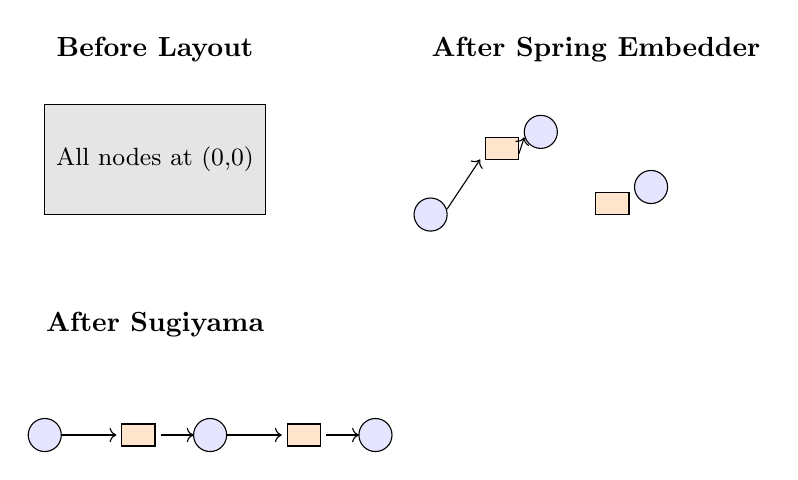
\begin{tikzpicture}[scale=0.7]
        % Before layout
        \node at (-4, 3) {\textbf{Before Layout}};
        \draw[fill=gray!20] (-6, 0) rectangle (-2, 2);
        \node at (-4, 1) {\small All nodes at (0,0)};
        
        % After Spring Embedder
        \node at (4, 3) {\textbf{After Spring Embedder}};
        \draw[fill=blue!10] (1, 0) circle (0.3);
        \draw[fill=blue!10] (3, 1.5) circle (0.3);
        \draw[fill=blue!10] (5, 0.5) circle (0.3);
        \draw[fill=orange!20] (2, 1) rectangle (2.6, 1.4);
        \draw[fill=orange!20] (4, 0) rectangle (4.6, 0.4);
        \draw[->] (1.3, 0.1) -- (1.9, 1);
        \draw[->] (2.6, 1.1) -- (2.7, 1.4);
        
        % After Sugiyama
        \node at (-4, -2) {\textbf{After Sugiyama}};
        \draw[fill=blue!10] (-6, -4) circle (0.3);
        \draw[fill=orange!20] (-4.6, -4.2) rectangle (-4, -3.8);
        \draw[fill=blue!10] (-3, -4) circle (0.3);
        \draw[fill=orange!20] (-1.6, -4.2) rectangle (-1, -3.8);
        \draw[fill=blue!10] (0, -4) circle (0.3);
        \draw[->] (-5.7, -4) -- (-4.7, -4);
        \draw[->] (-3.9, -4) -- (-3.3, -4);
        \draw[->] (-2.7, -4) -- (-1.7, -4);
        \draw[->] (-0.9, -4) -- (-0.3, -4);
    \end{tikzpicture}
    \caption{Layout algorithm results comparison}
    \label{fig:layout-comparison}
\end{figure}

\section{When to Use Which Algorithm}
\label{sec:layout-guidance}

\begin{itemize}
    \item \textbf{Spring Embedder}: 
    \begin{itemize}
        \item Petri nets with many cycles
        \item Organic, symmetric patterns
        \item When hierarchy is not important
    \end{itemize}
    
    \item \textbf{Sugiyama}: 
    \begin{itemize}
        \item Sequential, workflow-like processes
        \item When you want left-to-right or top-to-bottom flow
        \item PNML imports without layout data (default)
    \end{itemize}
\end{itemize}

\section{Summary}
\label{sec:layout-summary}

Layout algorithms transform cluttered diagrams into readable visualizations:

\begin{itemize}
    \item \textbf{Spring Embedder}: Physics-based, produces organic layouts
    \item \textbf{Sugiyama}: Four-phase hierarchical algorithm
    \begin{enumerate}
        \item Cycle removal (DFS-based)
        \item Layer assignment (longest path)
        \item Vertex ordering (barycenter method)
        \item Coordinate assignment
    \end{enumerate}
    \item Both algorithms modify the \texttt{position} property of nodes directly
    \item \texttt{triggerDataChanged(true)} notifies UI to redraw and fit content
\end{itemize}

The next chapter covers the \textbf{Planning Service}, which enables communication with the backend for simulation and analysis.

\chapter{Planning Service: Backend API Integration}
\label{chap:planning-service}

The previous chapters covered client-side functionality: UI state, data management, file I/O, and layout algorithms. This chapter introduces the \textbf{Planning Service}, which extends the application's capabilities by communicating with a powerful backend server for simulation and analysis tasks.

\section{Problem Statement}
\label{sec:planning-problem}

Some operations are too complex or resource-intensive for browser-based execution:

\begin{itemize}
    \item \textbf{Long simulations}: Running thousands of firing steps
    \item \textbf{Stochastic analysis}: Monte Carlo simulations with multiple runs
    \item \textbf{AI planning}: Computing optimal transition sequences
    \item \textbf{Domain-specific algorithms}: Offshore scheduling optimization
\end{itemize}

These tasks require:
\begin{itemize}
    \item More computing power than browsers provide
    \item Specialized libraries (e.g., Python's \texttt{gspn4py} for stochastic Petri nets)
    \item Server-side state management for long-running operations
\end{itemize}

The \texttt{PlanningService} acts as a \textbf{bridge} between the frontend and backend, sending requests and receiving results via HTTP.

\section{System Architecture}
\label{sec:planning-architecture}

\begin{figure}[htb]
    \centering
    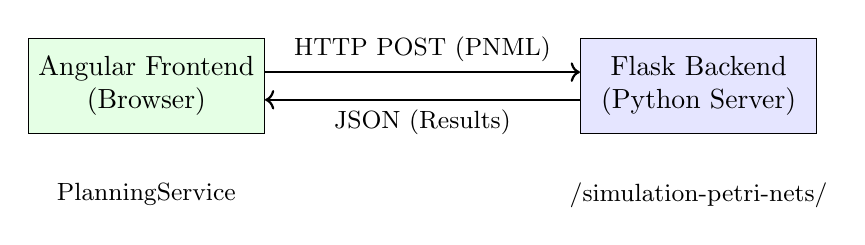
\begin{tikzpicture}[
        node distance=2cm,
        box/.style={rectangle, draw, minimum width=3cm, minimum height=1.2cm, align=center},
        arrow/.style={->, thick},
    ]
        % Frontend
        \node[box, fill=green!10] (fe) {Angular Frontend\\(Browser)};
        
        % Backend
        \node[box, fill=blue!10, right=4cm of fe] (be) {Flask Backend\\(Python Server)};
        
        % Arrows
        \draw[arrow] ([yshift=5pt]fe.east) -- node[above] {\small HTTP POST (PNML)} ([yshift=5pt]be.west);
        \draw[arrow] ([yshift=-5pt]be.west) -- node[below] {\small JSON (Results)} ([yshift=-5pt]fe.east);
        
        % Labels
        \node[below=0.5cm of fe] {\small PlanningService};
        \node[below=0.5cm of be] {\small /simulation-petri-nets/};
        
    \end{tikzpicture}
    \caption{Frontend-backend communication via PlanningService}
    \label{fig:planning-architecture}
\end{figure}

\section{Environment Configuration}
\label{sec:planning-environment}

The backend URL is configured via Angular's environment files:

\begin{lstlisting}[language=TypeScript, caption={Development environment (src/environments/environment.ts)}]
export const environment = {
    production: false,
    backendApiUrl: 'http://localhost:9040/l3s-offshore-2'
};
\end{lstlisting}

\begin{lstlisting}[language=TypeScript, caption={Production environment (src/environments/environment.prod.ts)}]
export const environment = {
    production: true,
    backendApiUrl: 'https://l3s-offshore-plan-2.l3s.uni-hannover.de/l3s-offshore-2'
};
\end{lstlisting}

Angular automatically swaps these files during the build process, ensuring development builds connect to \texttt{localhost} while production builds use the live server.

\section{PlanningService Implementation}
\label{sec:planning-implementation}

\begin{lstlisting}[language=TypeScript, caption={Planning service (src/app/tr-services/planning.service.ts)}]
import { Injectable } from '@angular/core';
import { HttpClient, HttpErrorResponse } from '@angular/common/http';
import { Observable, throwError } from 'rxjs';
import { catchError } from 'rxjs/operators';
import { environment } from '../../environments/environment';

@Injectable({
    providedIn: 'root'
})
export class PlanningService {
    /** Base URL for planning-related endpoints */
    private apiUrl = `${environment.backendApiUrl}/dto/planning`;
    
    /** URL for Petri net simulation endpoints */
    private simpleSimApiUrl = `${environment.backendApiUrl}/simulation-petri-nets/simple-sim`;

    constructor(private http: HttpClient) {}

    // =========================================================================
    // SIMULATION METHODS
    // =========================================================================

    /**
     * Run a Petri net simulation on the backend.
     * Sends the PNML file and receives firing sequence results.
     * 
     * @param pnmlFile - The PNML file to simulate
     * @param runs - Number of simulation runs (for stochastic analysis)
     * @returns Observable with simulation results
     */
    runSimpleSimulation(pnmlFile: File, runs: number = 1): Observable<SimulationResult> {
        // FormData is required for file uploads
        const formData = new FormData();
        formData.append('pnml_model', pnmlFile, pnmlFile.name);
        formData.append('num_runs', runs.toString());

        return this.http.post<SimulationResult>(this.simpleSimApiUrl, formData)
            .pipe(catchError(this.handleError));
    }

    /**
     * Convenience method: run simulation from PNML string.
     * Converts the string to a File object before sending.
     */
    runSimpleSimulationFromString(
        pnmlContent: string, 
        runs: number = 1, 
        fileName: string = 'model.pnml'
    ): Observable<SimulationResult> {
        // Create a File from the string content
        const pnmlFile = new File([pnmlContent], fileName, { type: 'application/xml' });
        return this.runSimpleSimulation(pnmlFile, runs);
    }

    // =========================================================================
    // PARAMETER & CONFIGURATION METHODS
    // =========================================================================

    /**
     * Fetch default parameter values from backend.
     * Used to populate the parameter table with sensible defaults.
     */
    getDefaults(): Observable<ParameterDefaults> {
        return this.http.get<ParameterDefaults>(`${this.apiUrl}/defaults`)
            .pipe(catchError(this.handleError));
    }

    /**
     * Submit planning parameters to backend.
     * Triggers the offshore scheduling optimization.
     */
    runPlanning(planningData: PlanningRequest): Observable<PlanningResult> {
        return this.http.post<PlanningResult>(this.apiUrl, planningData)
            .pipe(catchError(this.handleError));
    }

    // =========================================================================
    // EXAMPLE MODEL METHODS
    // =========================================================================

    /**
     * Get list of available example models from backend.
     * Returns filenames like ["example1.pnml", "example2.pnml"]
     */
    getAvailableExampleModels(): Observable<string[]> {
        const url = `${environment.backendApiUrl}/simulation-petri-nets/example-models`;
        return this.http.get<string[]>(url)
            .pipe(catchError(this.handleError));
    }

    /**
     * Load a specific example model by name.
     * Returns the raw PNML content as a string.
     */
    loadExampleModelByName(name: string): Observable<string> {
        const url = `${environment.backendApiUrl}/simulation-petri-nets/example-models/${encodeURIComponent(name)}`;
        return this.http.get(url, { responseType: 'text' })
            .pipe(catchError(this.handleError));
    }

    // =========================================================================
    // ERROR HANDLING
    // =========================================================================

    /**
     * Centralized error handler for all HTTP requests.
     * Logs the error and returns a user-friendly Observable error.
     */
    private handleError(error: HttpErrorResponse): Observable<never> {
        let message: string;

        if (error.error instanceof ErrorEvent) {
            // Client-side error (network issues, etc.)
            message = `Network error: ${error.error.message}`;
        } else {
            // Server-side error
            message = `Server error: ${error.status} - ${error.message}`;
        }

        console.error('[PlanningService]', message);
        return throwError(() => new Error(message));
    }
}

// =========================================================================
// TYPE DEFINITIONS
// =========================================================================

interface SimulationResult {
    /** Sequence of transition IDs that fired */
    firing_seq: string[];
    /** Token counts at each step (optional) */
    detailed_log?: StepLog[];
    /** Statistics for multi-run simulations */
    statistics?: TransitionStats;
}

interface StepLog {
    step: number;
    transition: string;
    marking: { [placeId: string]: number };
}

interface TransitionStats {
    [transitionId: string]: {
        fire_count: number;
        fire_percentage: number;
    };
}

interface ParameterDefaults {
    [paramName: string]: number | string | boolean;
}

interface PlanningRequest {
    model_pnml: string;
    parameters: { [key: string]: any };
}

interface PlanningResult {
    schedule: any[];
    metrics: { [key: string]: number };
}
\end{lstlisting}

\section{Usage in Components}
\label{sec:planning-usage}

\subsection{Running a Simulation}

\begin{lstlisting}[language=TypeScript, caption={Using PlanningService in ButtonBarComponent}]
import { Component } from '@angular/core';
import { PlanningService } from '../../tr-services/planning.service';
import { PnmlService } from '../../tr-services/pnml.service';
import { UiService } from '../../tr-services/ui.service';

@Component({ /* ... */ })
export class ButtonBarComponent {
    constructor(
        private planningService: PlanningService,
        private pnmlService: PnmlService,
        private uiService: UiService
    ) {}

    /**
     * Called when user clicks "Run Simulation" button.
     */
    runSimulation(): void {
        // 1. Get current Petri net as PNML string
        const pnmlContent = this.pnmlService.getPNML();

        // 2. Send to backend for simulation
        this.planningService
            .runSimpleSimulationFromString(pnmlContent, 1)
            .subscribe({
                next: (result) => {
                    console.log('Simulation complete:', result.firing_seq.length, 'steps');
                    
                    // 3. Update UI with results
                    this.uiService.setSimulationResults(result);
                    this.uiService.tab = TabState.Simulation;
                },
                error: (err) => {
                    console.error('Simulation failed:', err.message);
                    this.showErrorDialog('Simulation failed: ' + err.message);
                }
            });
    }
}
\end{lstlisting}

\subsection{Loading Example Models}

\begin{lstlisting}[language=TypeScript, caption={Loading example models with dropdown}]
import { Component, OnInit } from '@angular/core';
import { Observable } from 'rxjs';
import { PlanningService } from '../../tr-services/planning.service';
import { PnmlService } from '../../tr-services/pnml.service';

@Component({
    selector: 'app-example-selector',
    template: `
        <select (change)="onModelSelected($event)">
            <option value="">-- Select Example --</option>
            <option *ngFor="let model of availableModels$ | async" [value]="model">
                {{ model }}
            </option>
        </select>
    `
})
export class ExampleSelectorComponent implements OnInit {
    availableModels$: Observable<string[]>;

    constructor(
        private planningService: PlanningService,
        private pnmlService: PnmlService
    ) {}

    ngOnInit(): void {
        // Fetch available examples on component init
        this.availableModels$ = this.planningService.getAvailableExampleModels();
    }

    onModelSelected(event: Event): void {
        const select = event.target as HTMLSelectElement;
        const modelName = select.value;

        if (!modelName) return;

        // Load the selected model
        this.planningService.loadExampleModelByName(modelName).subscribe({
            next: (pnmlContent) => {
                // Parse and load into DataService
                this.pnmlService.parse(pnmlContent);
                console.log('Loaded example:', modelName);
            },
            error: (err) => {
                console.error('Failed to load example:', err.message);
            }
        });
    }
}
\end{lstlisting}

\section{Request/Response Flow}
\label{sec:planning-flow}

\begin{figure}[htb]
    \centering
    \begin{tikzpicture}[
        node distance=1.2cm,
        box/.style={rectangle, draw, minimum width=2.2cm, minimum height=0.6cm, font=\small},
    ]
        % Actors
        \node[box] (user) at (0,0) {User};
        \node[box] (btn) at (3,0) {ButtonBar};
        \node[box] (pnml) at (6,0) {PnmlService};
        \node[box] (plan) at (9,0) {PlanningService};
        \node[box] (back) at (12,0) {Backend};
        
        % Flow
        \draw[->] (user) -- ++(0,-1) -| node[pos=0.25, below] {\tiny clicks Run} (btn);
        \draw[->] (btn) -- ++(0,-2) -| node[pos=0.25, below] {\tiny getPNML()} (pnml);
        \draw[->] (pnml) -- ++(0,-3) -| node[pos=0.25, below] {\tiny PNML string} (btn);
        \draw[->] (btn) -- ++(0,-4) -| node[pos=0.25, below] {\tiny runSimulation()} (plan);
        \draw[->] (plan) -- ++(0,-5) -| node[pos=0.25, below] {\tiny POST /simple-sim} (back);
        \draw[->] (back) -- ++(0,-6) -| node[pos=0.25, below] {\tiny JSON result} (plan);
        \draw[->] (plan) -- ++(0,-7) -| node[pos=0.25, below] {\tiny Observable<Result>} (btn);
        
    \end{tikzpicture}
    \caption{Simulation request flow through PlanningService}
    \label{fig:simulation-flow}
\end{figure}

\section{Backend API Endpoints}
\label{sec:planning-endpoints}

The backend exposes the following REST endpoints:

\begin{table}[htb]
    \centering
    \begin{tabular}{llp{6cm}}
        \toprule
        \textbf{Method} & \textbf{Endpoint} & \textbf{Description} \\
        \midrule
        GET & \texttt{/dto/planning/defaults} & Get default parameter values \\
        POST & \texttt{/dto/planning} & Run planning optimization \\
        POST & \texttt{/simulation-petri-nets/simple-sim} & Run Petri net simulation \\
        GET & \texttt{/simulation-petri-nets/example-models} & List available examples \\
        GET & \texttt{/simulation-petri-nets/example-models/:name} & Get example PNML content \\
        \bottomrule
    \end{tabular}
    \caption{Backend API endpoints}
    \label{tab:api-endpoints}
\end{table}

\section{Error Handling Patterns}
\label{sec:planning-errors}

Robust error handling ensures graceful degradation when the backend is unavailable:

\begin{lstlisting}[language=TypeScript, caption={Error handling with retry and fallback}]
import { catchError, retry, timeout } from 'rxjs/operators';
import { of } from 'rxjs';

// With retry and timeout
this.planningService.runSimpleSimulation(file)
    .pipe(
        timeout(30000),  // 30 second timeout
        retry(2),        // Retry twice on failure
        catchError(err => {
            // Fallback to empty result
            console.warn('Simulation failed, using empty result');
            return of({ firing_seq: [], detailed_log: [] });
        })
    )
    .subscribe(result => {
        // Handle result (real or fallback)
    });
\end{lstlisting}

\section{CORS Configuration}
\label{sec:planning-cors}

For development, the backend must allow cross-origin requests from the Angular dev server:

\begin{lstlisting}[language=Python, caption={Flask CORS configuration (backend)}]
from flask import Flask
from flask_cors import CORS

app = Flask(__name__)
CORS(app, resources={
    r"/l3s-offshore-2/*": {
        "origins": ["http://localhost:4200"],
        "methods": ["GET", "POST", "OPTIONS"],
        "allow_headers": ["Content-Type"]
    }
})
\end{lstlisting}

In production, the nginx reverse proxy handles CORS headers.

\section{Summary}
\label{sec:planning-summary}

The \texttt{PlanningService} extends frontend capabilities through backend communication:

\begin{itemize}
    \item \textbf{HTTP Communication}: Uses Angular's \texttt{HttpClient} for REST API calls
    \item \textbf{Environment Configuration}: Separate URLs for development and production
    \item \textbf{File Uploads}: Uses \texttt{FormData} to send PNML files
    \item \textbf{Error Handling}: Centralized handler with user-friendly messages
    \item \textbf{Observable Pattern}: Async results via RxJS Observables
\end{itemize}

This service enables the application to leverage powerful server-side algorithms while maintaining a responsive, client-side user interface.


% Part V: Deployment and Conclusion
\chapter{Deployment}
\label{chap:deployment}

This chapter describes how to build and deploy the L3S-Offshore-2 Frontend, both locally for development and on production servers.

\section{Prerequisites}
\label{sec:prerequisites}

\subsection{Development Environment}

The following software is required for local development:

\begin{itemize}
    \item \textbf{Node.js:} Version 18.x or higher (LTS recommended)
    \item \textbf{npm:} Version 9.x or higher (comes with Node.js)
    \item \textbf{Angular CLI:} Version 17.x (\texttt{npm install -g @angular/cli})
    \item \textbf{Git:} For version control
\end{itemize}

\subsection{Production Environment}

For production deployment:

\begin{itemize}
    \item \textbf{Docker:} Version 20.x or higher
    \item \textbf{Docker Compose:} (optional, for multi-container setups)
    \item \textbf{nginx:} Included in the Docker image
\end{itemize}

\section{Local Development}
\label{sec:local-development}

\subsection{Clone and Install}

\begin{lstlisting}[language=bash, caption={Cloning and installing dependencies}]
# Clone the repository
git clone https://github.com/krausality/PNML_Frontend.git
cd PNML_Frontend

# Install dependencies
npm install
\end{lstlisting}

\subsection{Development Server}

Start the Angular development server with hot reloading:

\begin{lstlisting}[language=bash, caption={Starting the development server}]
# Start development server
ng serve

# Or with explicit host binding (for network access)
ng serve --host 0.0.0.0 --port 4200
\end{lstlisting}

The application will be available at \url{http://localhost:4200}.

\subsection{Backend Connection}

The development environment expects the Flask backend to run on port 9040. Configure the backend URL in \texttt{src/environments/environment.ts}:

\begin{lstlisting}[language=TypeScript, caption={Development environment configuration}]
export const environment = {
  production: false,
  apiUrl: 'http://localhost:9040'
};
\end{lstlisting}

\section{Production Build}
\label{sec:production-build}

\subsection{Angular Production Build}

Create an optimized production build:

\begin{lstlisting}[language=bash, caption={Creating a production build}]
# Production build with optimizations
ng build --configuration production

# Output is generated in dist/pnml-frontend/
\end{lstlisting}

The production build includes:
\begin{itemize}
    \item Ahead-of-Time (AOT) compilation
    \item Tree shaking to remove unused code
    \item Minification and uglification
    \item Content hashing for cache busting
\end{itemize}

\subsection{Build Verification}

Verify the build output:

\begin{lstlisting}[language=bash, caption={Verifying the production build}]
# Check bundle sizes
ls -la dist/pnml-frontend/browser/

# Expected output: main.js, polyfills.js, styles.css
# Total size should be under 500KB gzipped
\end{lstlisting}

\section{Docker Deployment}
\label{sec:docker-deployment}

\subsection{Dockerfile}

The application uses a multi-stage Dockerfile:

\begin{lstlisting}[language=docker, caption={Multi-stage Dockerfile}]
# Stage 1: Build
FROM node:18-alpine AS builder
WORKDIR /app
COPY package*.json ./
RUN npm ci
COPY . .
RUN npm run build -- --configuration production

# Stage 2: Serve with nginx
FROM nginx:alpine
COPY --from=builder /app/dist/pnml-frontend/browser /usr/share/nginx/html
COPY nginx.conf /etc/nginx/nginx.conf
EXPOSE 80
CMD ["nginx", "-g", "daemon off;"]
\end{lstlisting}

\subsection{Nginx Configuration}

The nginx configuration handles SPA routing:

\begin{lstlisting}[caption={nginx.conf for SPA routing}]
server {
    listen 80;
    server_name localhost;
    root /usr/share/nginx/html;
    index index.html;
    
    # SPA fallback: serve index.html for all routes
    location / {
        try_files $uri $uri/ /index.html;
    }
    
    # Cache static assets
    location ~* \.(js|css|png|jpg|jpeg|gif|ico|svg|woff|woff2)$ {
        expires 1y;
        add_header Cache-Control "public, immutable";
    }
    
    # Gzip compression
    gzip on;
    gzip_types text/plain text/css application/json application/javascript;
}
\end{lstlisting}

\subsection{Building the Docker Image}

\begin{lstlisting}[language=bash, caption={Building and running the Docker container}]
# Build the image
docker build -t l3s-offshore-frontend:latest .

# Run the container
docker run -d -p 8080:80 --name offshore-frontend l3s-offshore-frontend:latest

# Verify it's running
curl http://localhost:8080
\end{lstlisting}

\section{Server Deployment}
\label{sec:server-deployment}

\subsection{L3S Infrastructure}

The L3S research infrastructure uses a nested VPS architecture. Access requires:

\begin{enumerate}
    \item SSH to the gateway server (\texttt{gate.l3s.uni-hannover.de})
    \item SSH to the project VPS
    \item Docker commands within the VPS
\end{enumerate}

\subsection{Deployment Script}

A typical deployment workflow:

\begin{lstlisting}[language=bash, caption={Production deployment script}]
#!/bin/bash
# deploy.sh

# 1. Build and push to container registry
docker build -t registry.l3s.de/offshore/frontend:latest .
docker push registry.l3s.de/offshore/frontend:latest

# 2. On the server: pull and restart
ssh user@server << 'EOF'
  docker pull registry.l3s.de/offshore/frontend:latest
  docker stop offshore-frontend || true
  docker rm offshore-frontend || true
  docker run -d -p 80:80 --name offshore-frontend \
    registry.l3s.de/offshore/frontend:latest
EOF
\end{lstlisting}

\subsection{Docker Cleanup}

After deployment, clean up old images to save disk space:

\begin{lstlisting}[language=bash, caption={Docker cleanup commands}]
# Remove unused images (not just containers)
docker image prune -a --filter "until=24h"

# Remove stopped containers
docker container prune

# Full cleanup (use with caution)
docker system prune -a
\end{lstlisting}

\section{Environment Configuration}
\label{sec:environment-configuration}

\subsection{Production Environment}

Update \texttt{src/environments/environment.prod.ts} with production URLs:

\begin{lstlisting}[language=TypeScript, caption={Production environment configuration}]
export const environment = {
  production: true,
  apiUrl: 'https://api.offshore.l3s.de'
};
\end{lstlisting}

\subsection{Runtime Configuration}

For dynamic configuration without rebuilding, environment variables can be injected at container runtime:

\begin{lstlisting}[language=bash, caption={Runtime environment injection}]
docker run -d -p 80:80 \
  -e API_URL=https://new-api.example.com \
  l3s-offshore-frontend:latest
\end{lstlisting}

\section{Troubleshooting}
\label{sec:troubleshooting}

\subsection{Common Issues}

\begin{description}
    \item[Blank page after deployment:] Check nginx configuration and ensure \texttt{try\_files} fallback is configured for SPA routing.
    
    \item[API connection refused:] Verify the backend URL in environment configuration and check CORS settings on the backend.
    
    \item[Assets not loading:] Ensure \texttt{base href} in \texttt{index.html} matches the deployment path.
    
    \item[Container exits immediately:] Check logs with \texttt{docker logs <container-id>} and verify nginx configuration syntax.
\end{description}

\subsection{Logging}

Access container logs for debugging:

\begin{lstlisting}[language=bash, caption={Viewing container logs}]
# Follow logs in real-time
docker logs -f offshore-frontend

# Last 100 lines
docker logs --tail 100 offshore-frontend
\end{lstlisting}

\chapter{Related Work}
\label{chap:related-work}

This chapter discusses existing tools and approaches for Petri net visualization and simulation, and positions the L3S-Offshore-2 Frontend within this landscape.

\section{Desktop Petri Net Tools}
\label{sec:desktop-tools}

\subsection{WoPeD (Workflow Petri Net Designer)}

WoPeD is a widely-used open-source tool for editing and analyzing Workflow Petri nets. It provides:

\begin{itemize}
    \item Graphical editor for place/transition nets
    \item Structural analysis (e.g., place invariants)
    \item Token game simulation
    \item PNML import/export
\end{itemize}

\textbf{Comparison:} Unlike WoPeD, the L3S-Offshore-2 Frontend runs entirely in the browser, enabling collaboration without software installation. However, WoPeD offers more advanced analysis algorithms.

\subsection{CPN Tools}

CPN Tools is a tool for editing, simulating, and analyzing Colored Petri Nets (CPNs). It provides hierarchical modeling and state space analysis.

\textbf{Comparison:} CPN Tools supports more expressive Petri net types but requires desktop installation. The L3S frontend focuses on simpler P/T nets with web-based accessibility.

\section{Web-Based Petri Net Tools}
\label{sec:web-tools}

\subsection{i-love-petrinets (Original Fork)}

The L3S-Offshore-2 Frontend is based on a fork of the \texttt{i-love-petrinets} project, an Angular-based PNML viewer. The original provided:

\begin{itemize}
    \item PNML parsing and basic visualization
    \item Drag-and-drop editing
    \item Place invariant analysis
\end{itemize}

\textbf{Extensions in this project:}
\begin{itemize}
    \item Backend integration for simulation
    \item Animated firing sequence playback
    \item Offshore-specific parameter interface
    \item Production-ready deployment with Docker
    \item Significant UX improvements (zoom, pan, tab state management)
\end{itemize}

\subsection{Cytoscape.js}

Cytoscape.js is a general-purpose graph visualization library that has been extended for Petri nets. However, it lacks native PNML support and Petri net semantics.

\section{Simulation Backends}
\label{sec:simulation-backends}

\subsection{gspn4py}

The L3S backend uses \texttt{gspn4py}, a Python library for Generalized Stochastic Petri Nets. It provides:

\begin{itemize}
    \item Stochastic simulation with exponential delays
    \item Firing sequence generation
    \item Performance analysis
\end{itemize}

\subsection{pm4py}

pm4py is a Python library for process mining that also supports Petri net operations. It was considered during the project's initial phase but the focus shifted to custom simulation for offshore scheduling.

\section{Summary}

The L3S-Offshore-2 Frontend fills a niche for web-based Petri net visualization with domain-specific features for offshore logistics research. While desktop tools offer more advanced analysis, the web-based approach prioritizes accessibility and collaboration.
\chapter{Conclusion and Future Work}
\label{chap:conclusion}

This chapter summarizes the achievements of the L3S-Offshore-2 Frontend project and outlines directions for future development.

\section{Summary}
\label{sec:summary}

This documentation has described the development of a web-based frontend for Petri net visualization and simulation, created as part of the L3S-Offshore-2 research project.

\subsection{Achievements}

The following goals were accomplished:

\begin{enumerate}
    \item \textbf{Functional Visualization:} The application successfully renders Petri nets from PNML files with interactive editing capabilities.
    
    \item \textbf{Simulation Integration:} Full integration with the Flask backend enables multi-run simulations with firing sequence animation.
    
    \item \textbf{Offshore Parameter Interface:} A dedicated tab allows researchers to configure domain-specific parameters for scheduling models.
    
    \item \textbf{Production Deployment:} The application is containerized and deployed on L3S infrastructure, accessible via web browser.
    
    \item \textbf{Code Quality:} Extensive JSDoc documentation and English comments ensure maintainability for future developers.
\end{enumerate}

\subsection{Technical Highlights}

The most technically challenging aspects that were solved:

\begin{itemize}
    \item \textbf{Viewport-centered zoom:} Implementing intuitive zoom behavior with ResizeObserver integration
    \item \textbf{Tab-state management:} Ensuring UI consistency when switching between different workflows
    \item \textbf{Token reset logic:} Preserving initial markings across simulation runs
    \item \textbf{Reactive forms integration:} Solving performance issues with Angular's form system
\end{itemize}

\section{Limitations}
\label{sec:limitations}

The current implementation has the following limitations:

\begin{itemize}
    \item \textbf{No data persistence:} All data is stored in-memory and lost on page reload
    \item \textbf{Limited to P/T nets:} Higher-level Petri net types (colored, hierarchical) are not supported
    \item \textbf{Single-user:} No collaborative editing or user accounts
    \item \textbf{Visual overlaps:} Large nets may have overlapping elements with the current layout
\end{itemize}

\section{Future Work}
\label{sec:future-work}

The following enhancements could be pursued in future development:

\subsection{Short-Term (High Priority)}

\begin{itemize}
    \item \textbf{Interactive Miner Integration:} Connect to pm4py's interactive miner for process discovery
    \item \textbf{Analysis Endpoints:} Display conformance checking results from the backend
    \item \textbf{Export Functions:} Enable export of simulation results as CSV/JSON
\end{itemize}

\subsection{Medium-Term (Nice-to-Have)}

\begin{itemize}
    \item \textbf{Undo/Redo:} Implement history management for the Build tab
    \item \textbf{Data Persistence:} Add optional browser-based storage (IndexedDB)
    \item \textbf{Visual Improvements:} Reduce element overlaps with improved layout algorithms
\end{itemize}

\subsection{Long-Term (Research Extensions)}

\begin{itemize}
    \item \textbf{Colored Petri Nets:} Extend the data model and visualization for CPNs
    \item \textbf{Real-Time Monitoring:} WebSocket-based live updates during long-running simulations
    \item \textbf{Multi-User Collaboration:} Shared editing with conflict resolution
\end{itemize}

\section{Acknowledgements}
\label{sec:acknowledgements}

This project was developed at the L3S Research Center, Leibniz Universität Hannover, under the supervision of Peng Qian. The author thanks the original developers of the i-love-petrinets project for providing the initial codebase.

\appendix
\input{contents/A-appendix.tex}

\bibliographystyle{abbrv}
\bibliography{references}

\backmatter

\end{document}
